\section{Résultats}

Ici seront présentés les résultats des tests qui concernent le LiDAR Lite V4. Au fur et à mesure des
résultats, quelques conclusions seront d'ores et déjà tirées.\\
En annexe, se trouve le protocole de test complet du capteur.

\subsection{Caractéristique de l'erreur de mesure}

Le premier test consiste à mesurer une distance connue avec le capteur et de noter sa valeur mesurée
afin de vérifier si la plage de mesure donnée par la fiche technique (5cm à 10m) est vraie.\\
Ceci nous permet de savoir dans quelle mesure la distance fournie par le capteur représente la réalité.
Dans le cas d'une erreur de mesure, il nous est aussi utile de savoir si cette erreur est constante 
entre plusieurs séries espacées dans le temps.

\subsubsection{Méthode}

Pour ce faire, le capteur a été placé le long d'un étalon gradué de 6 mètres. Un objet est ensuite
placé à un interval de 20cm pour le premier mètre, puis à un interval de 50cm. À chaque mesure, on 
note la valeur mesurée par le LiDAR ainsi que la distance réelle.\\
Cela nous permet donc de comparer la plage de mesure effective du capteur, dans les tolérences
annoncées. La figure \ref{RealDistanceMeasures} montre la mise en place du test de distance.

\begin{figure}[H]
    \centering
    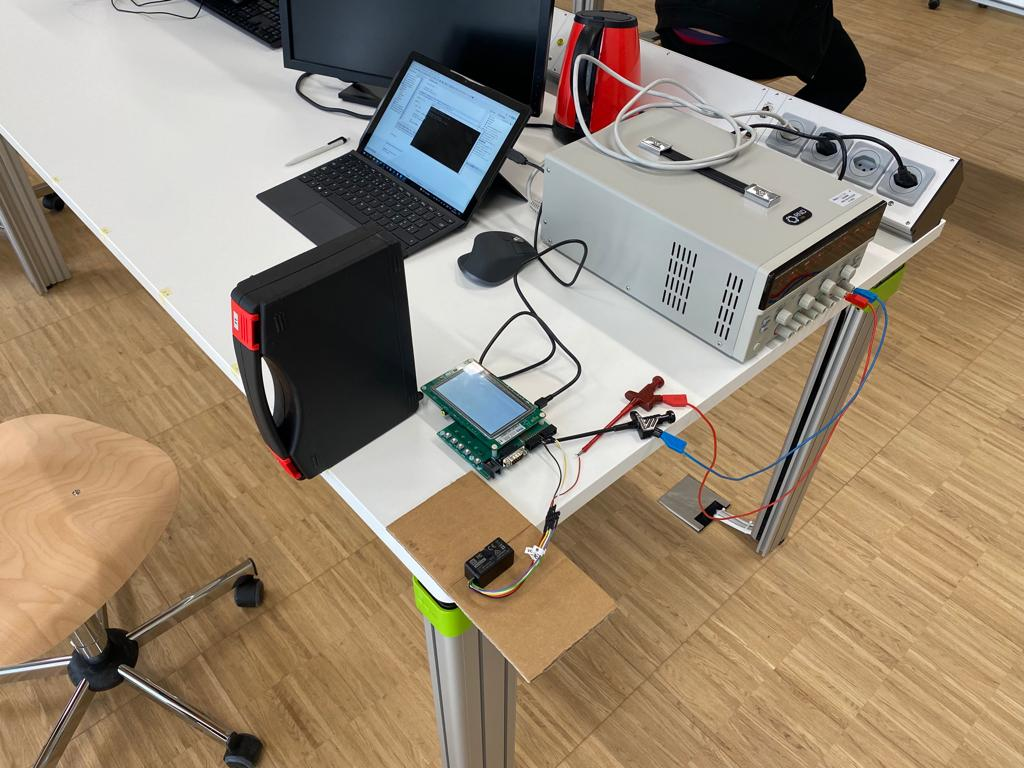
\includegraphics[width=0.5\textwidth]{Images/LiDAR/RealDistanceMes.jpeg}
    \caption{Mesure de distance comparée à la distance réelle}
    \label{RealDistanceMeasures}
\end{figure}

La mesure finale de distance est une moyenne de 10 mesures. Cela permet notamment d'éliminer partiellement
l'erreur due à la résolution finie du capteur.\\
Le test a été réalisé en intérieur, en l'absence total d'élément perturbateur, notamment de rayons 
infrarouges, à température ambiante (25°C).

\subsubsection{Résultats du test}

\begin{figure}[H]
    \centering
    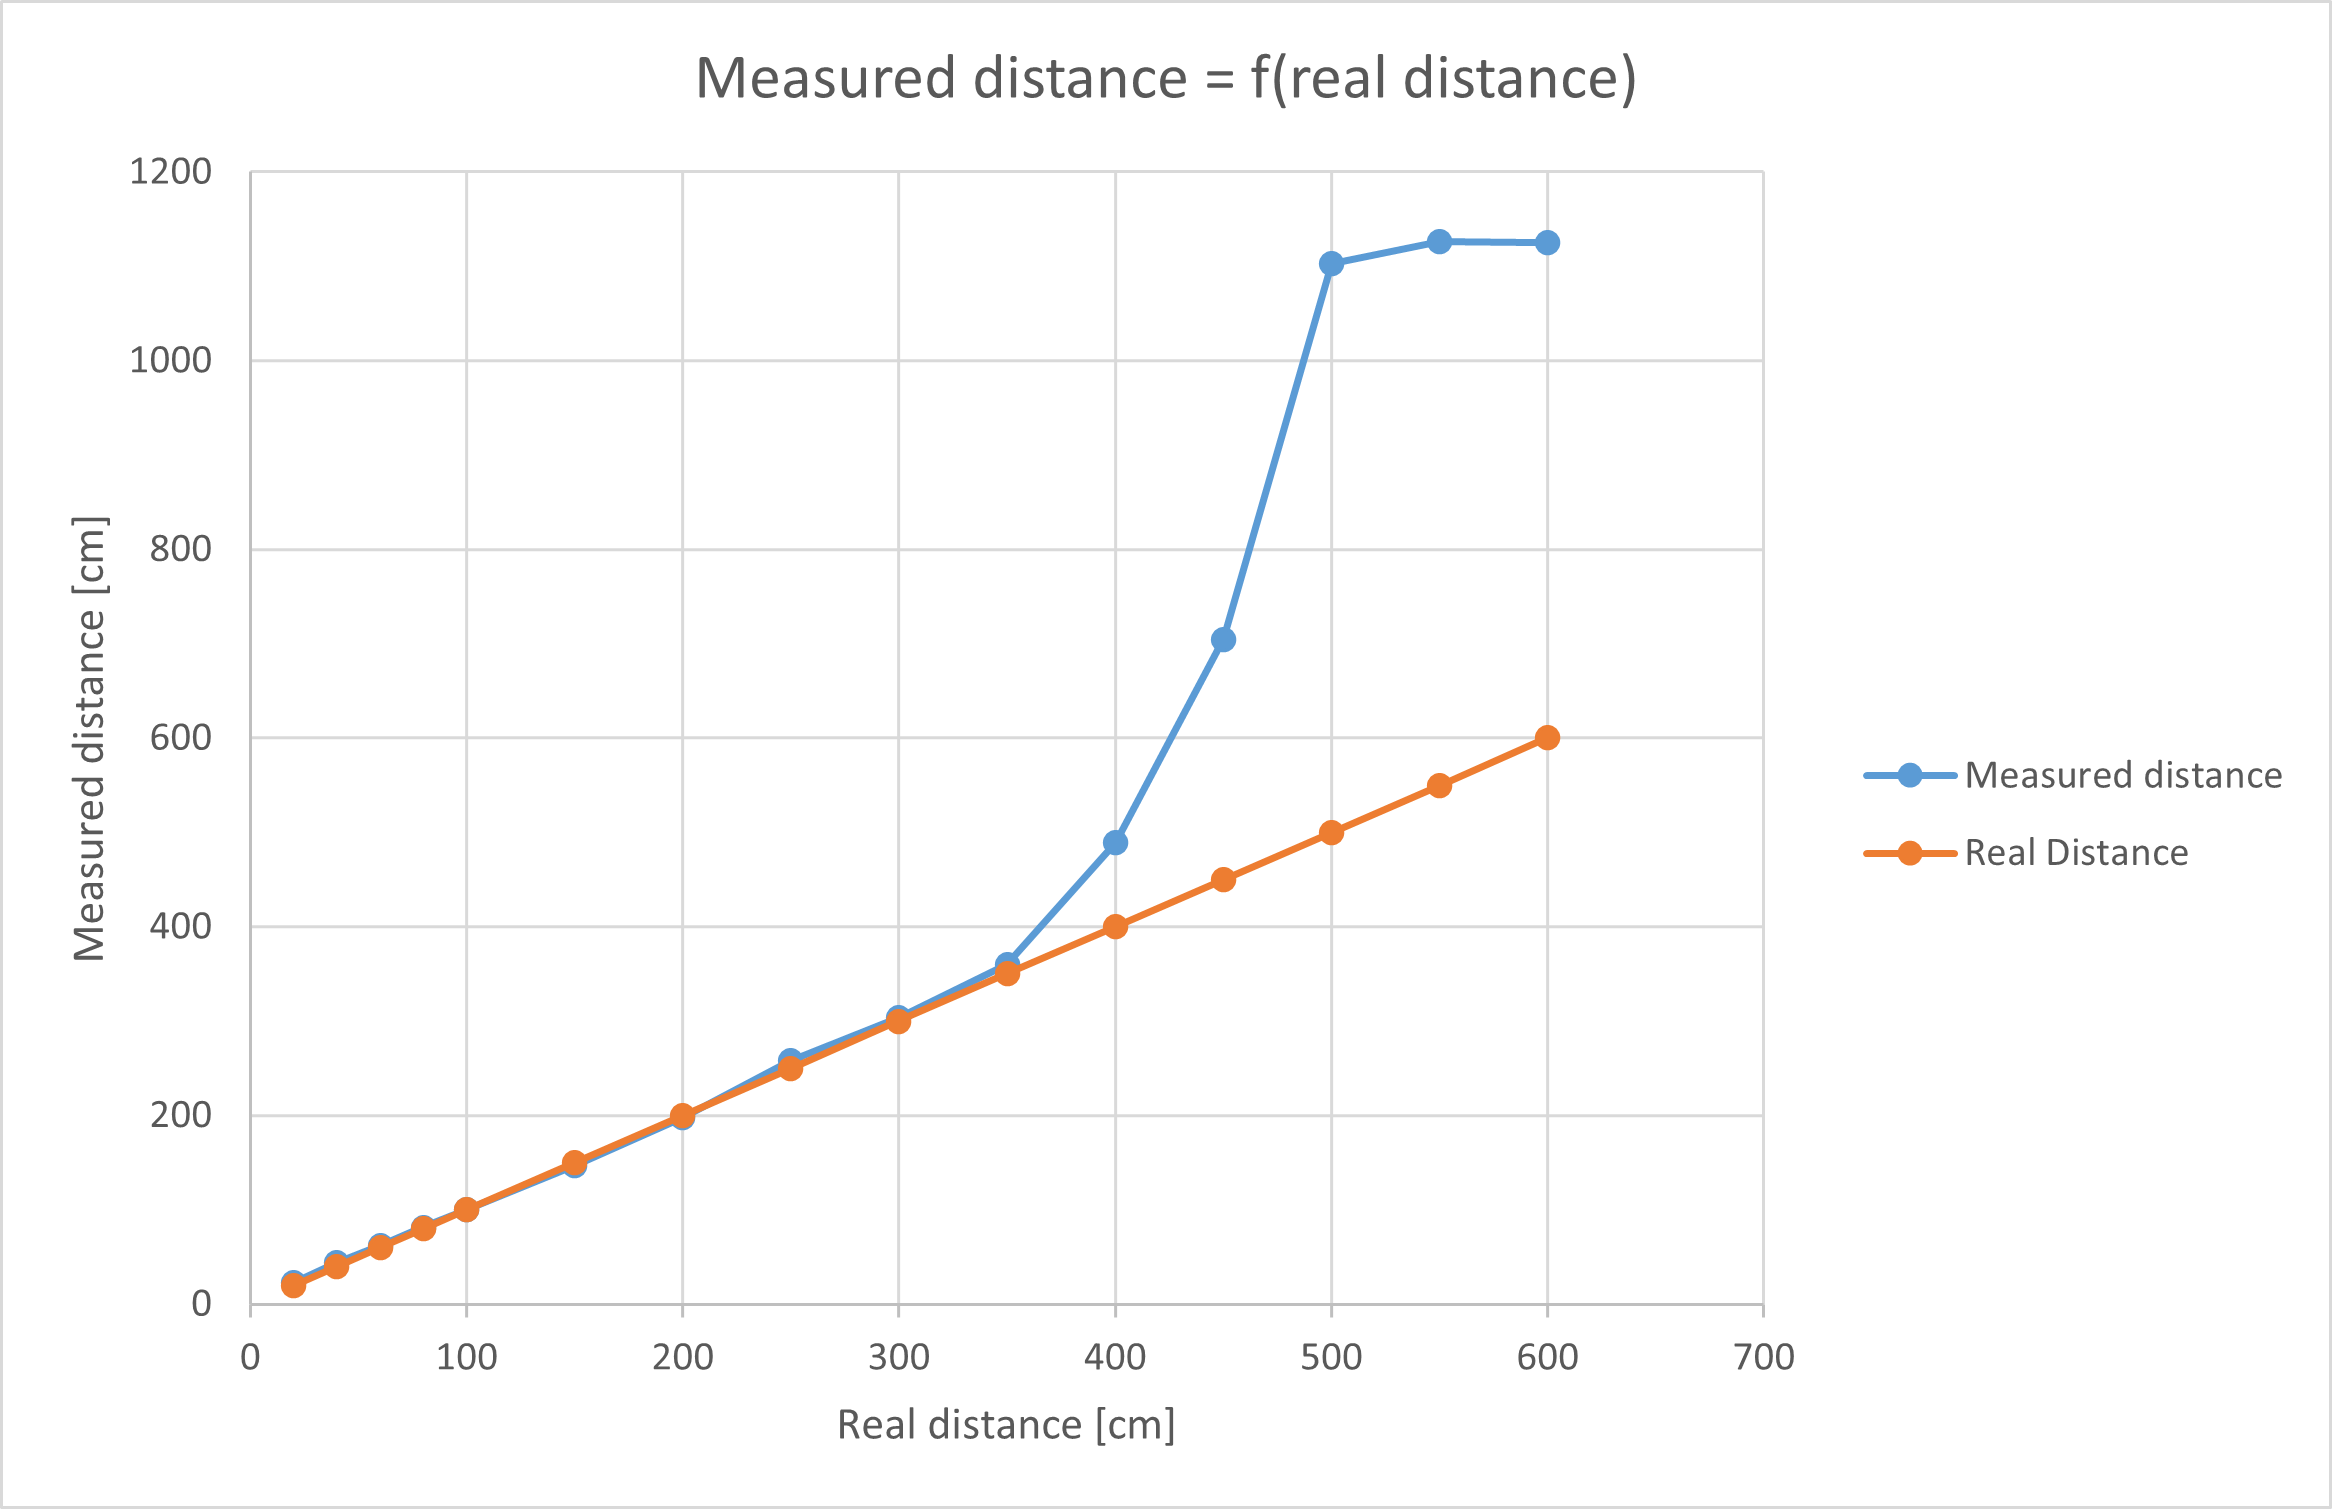
\includegraphics[width=0.8\textwidth]{Images/LiDAR/LiDARRealDistanceGraph_MesDist.png}
    \caption{Distance mesurée en fonction de la distance réelle}
    \label{RealDistanceMesGraph}
\end{figure}

\begin{figure}[H]
    \centering
    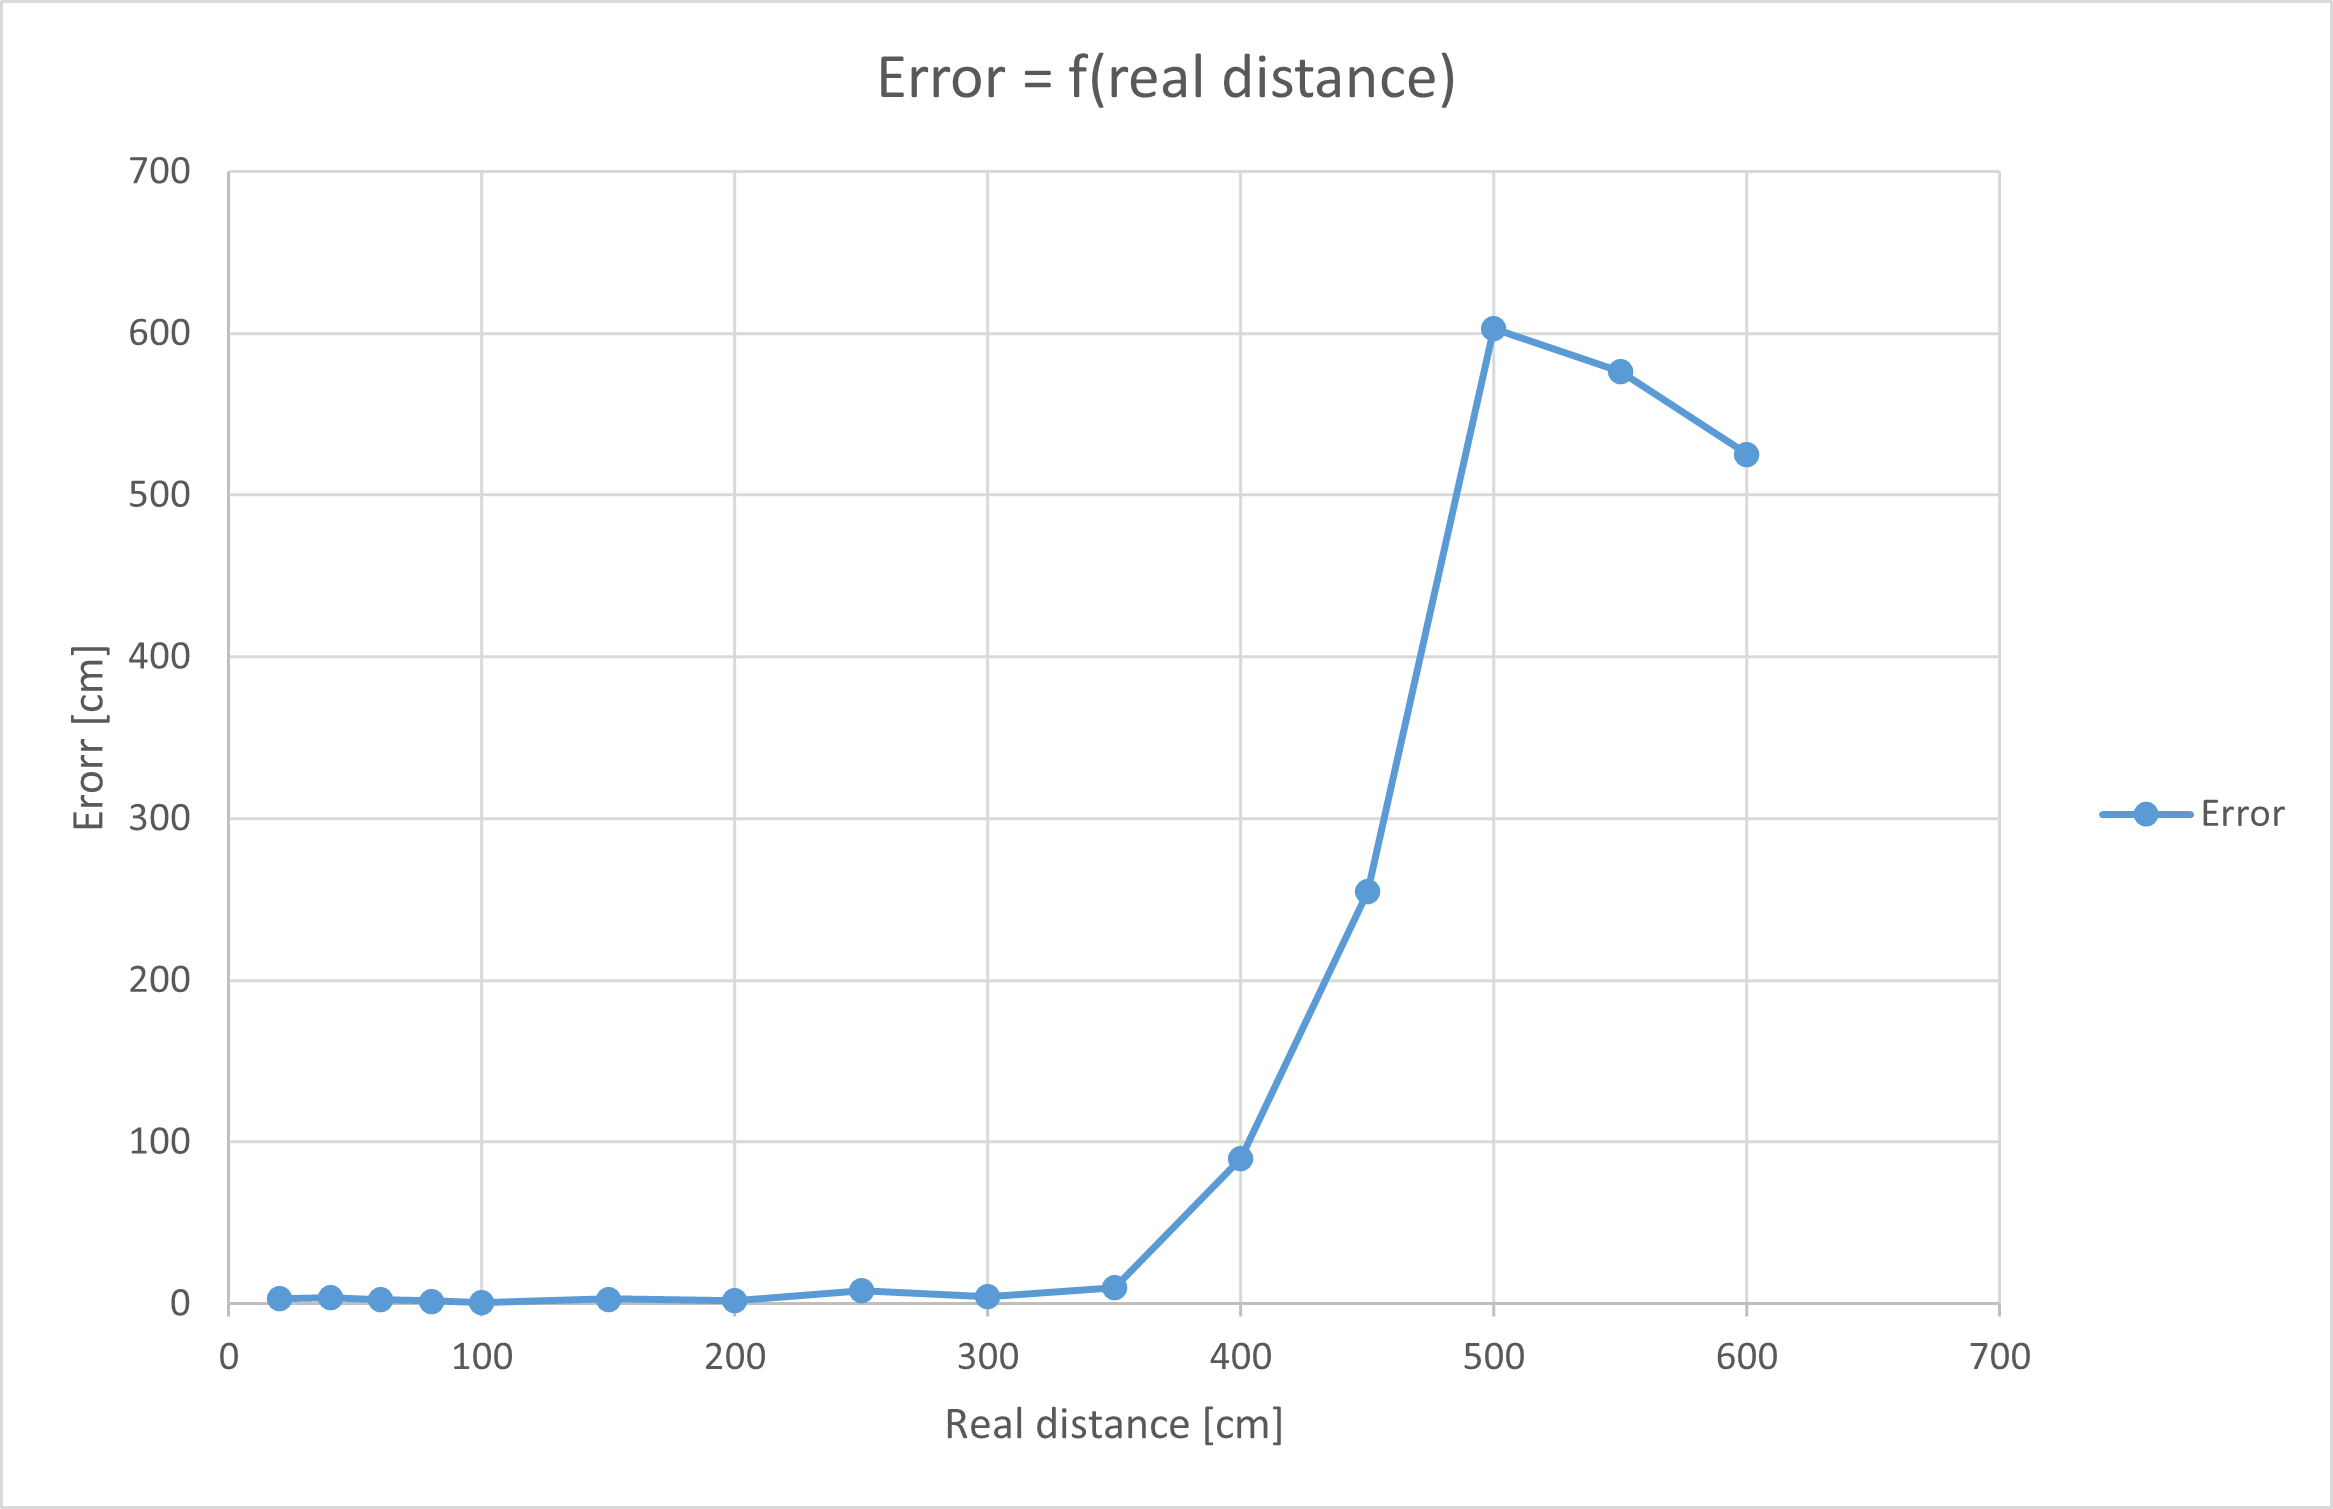
\includegraphics[width=0.8\textwidth]{Images/LiDAR/LiDARRealDistanceGraph_MesDistError.png}
    \caption{Erreur de la distance mesurée par rapport à la distance réelle}
    \label{RealDistanceMesGraphError}
\end{figure}

Nous avons jugé important de zoomer sur la plage utile entre 0 et 3m afin de visualiser les graphes 
de manière plus claire.

\begin{figure}[H]
    \centering
    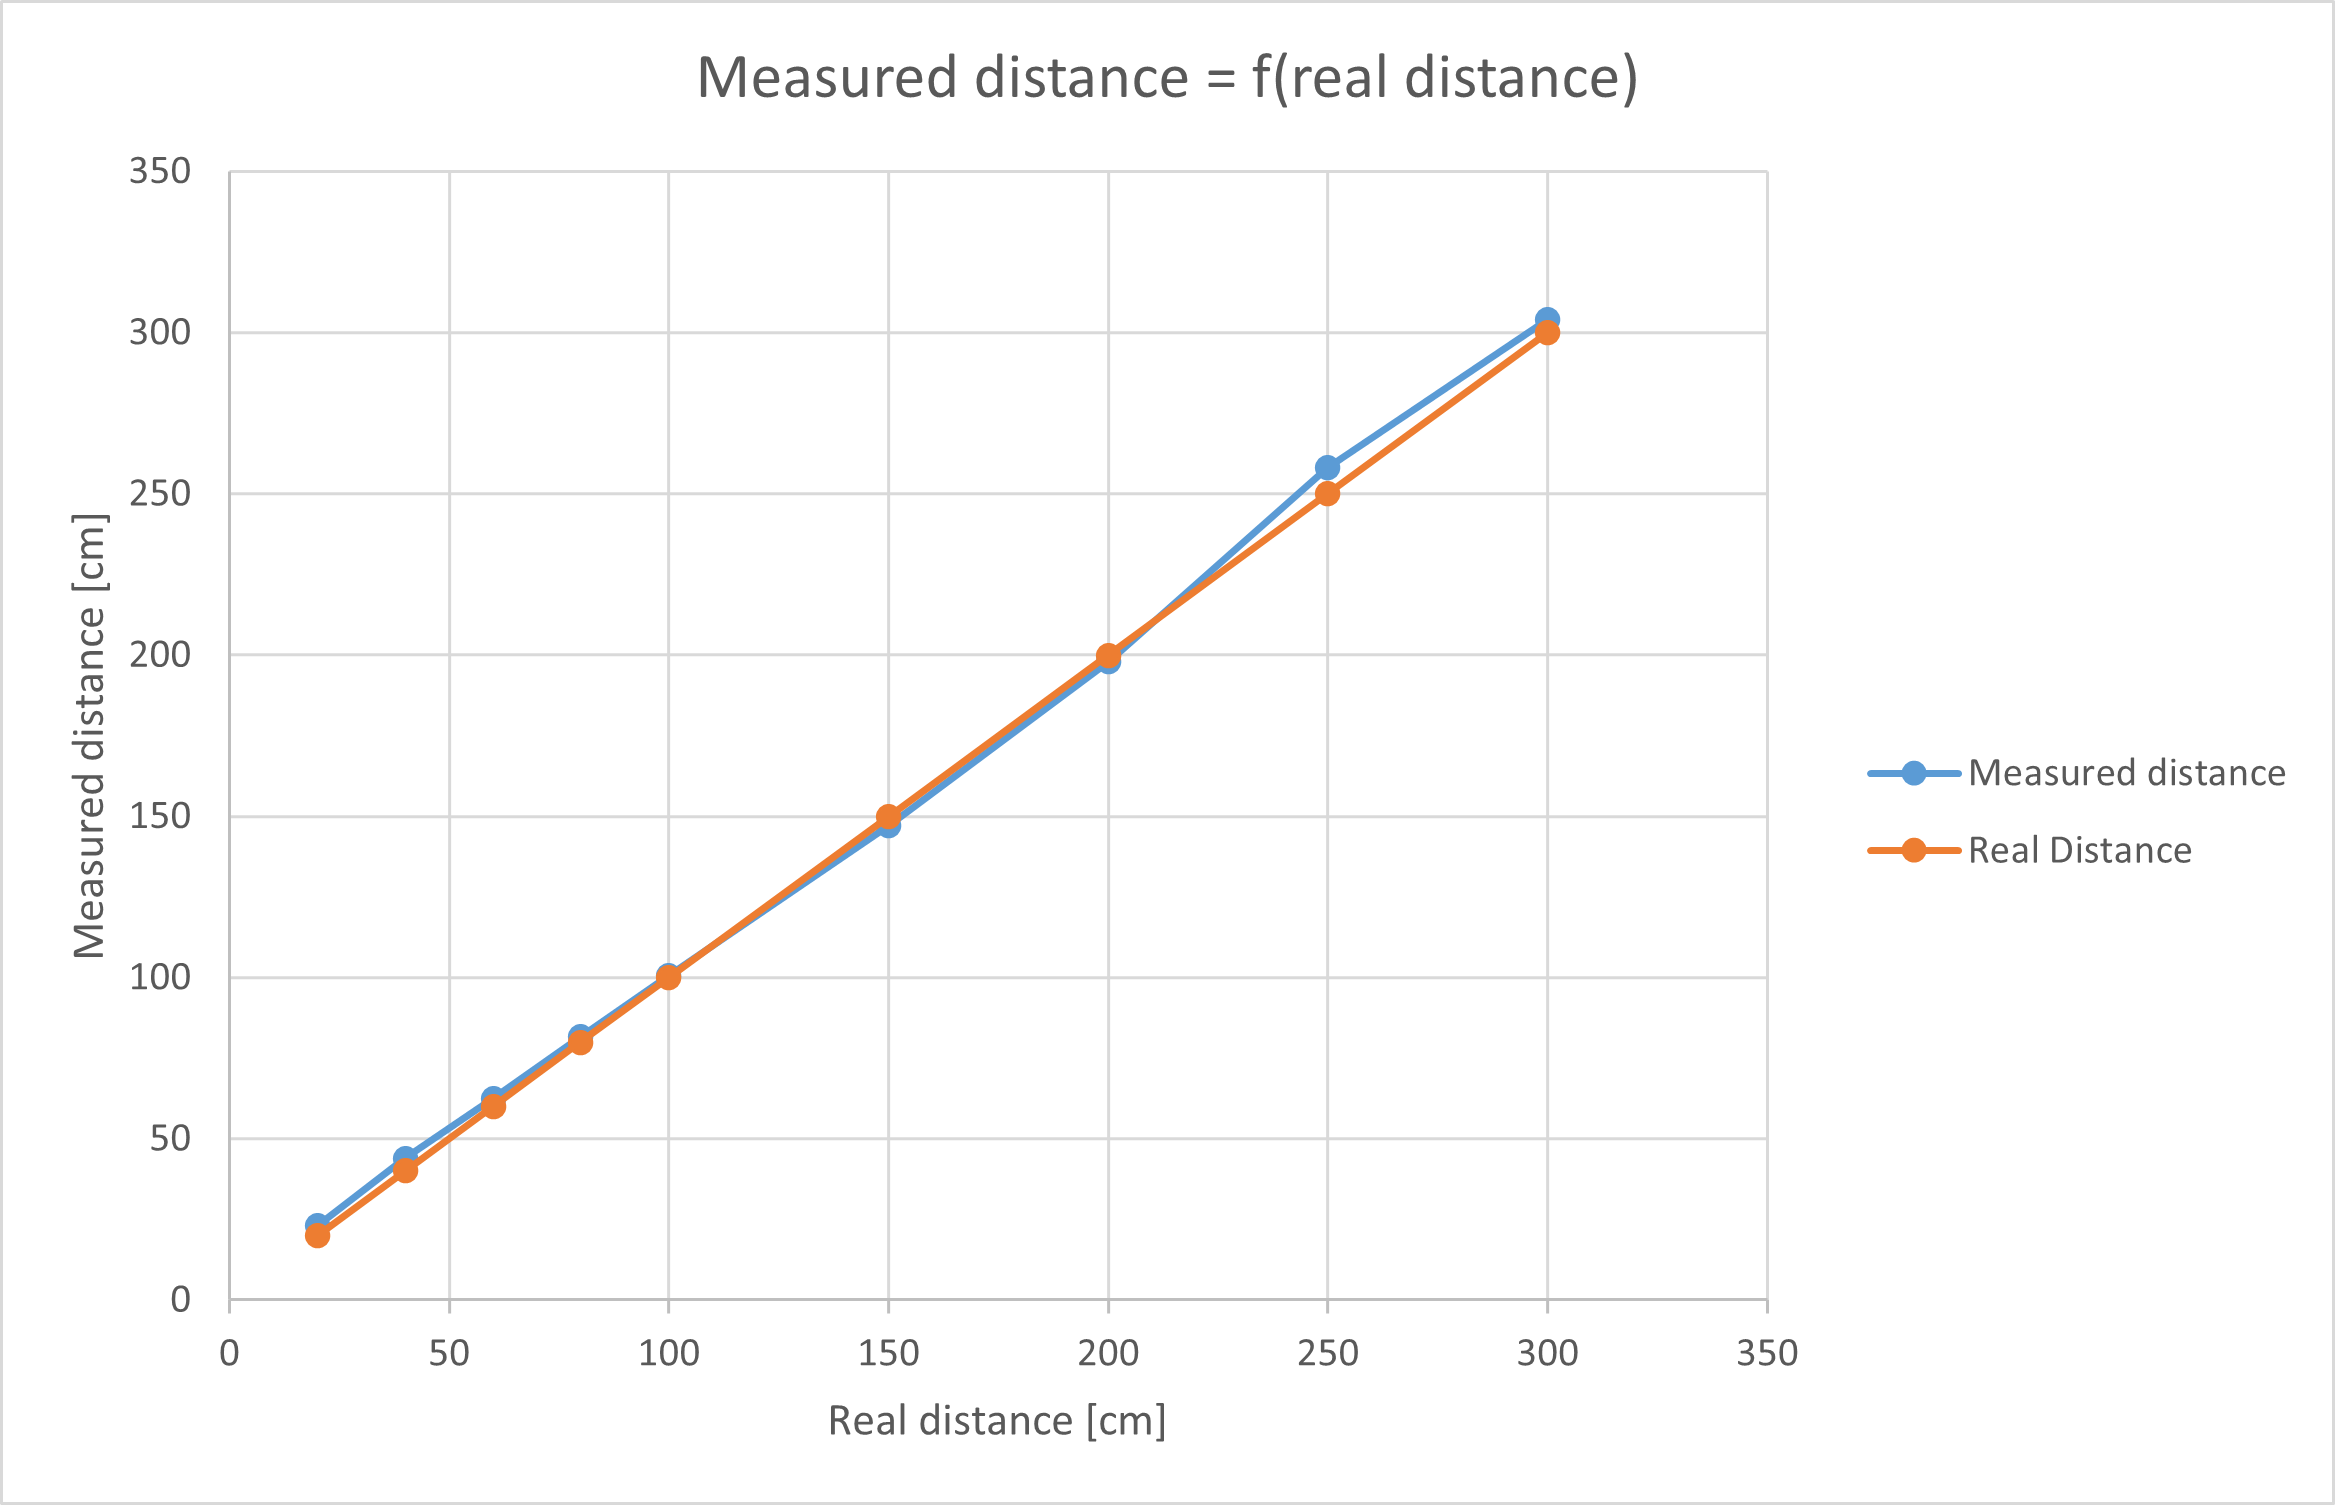
\includegraphics[width=0.8\textwidth]{Images/LiDAR/LiDARRealDistanceGraph_MesDist_Zoom.png}
    \caption{Distance mesurée en fonction de la distance réelle dans la plage utile}
    \label{RealDistanceMesGraphZoom}
\end{figure}

\begin{figure}[H]
    \centering
    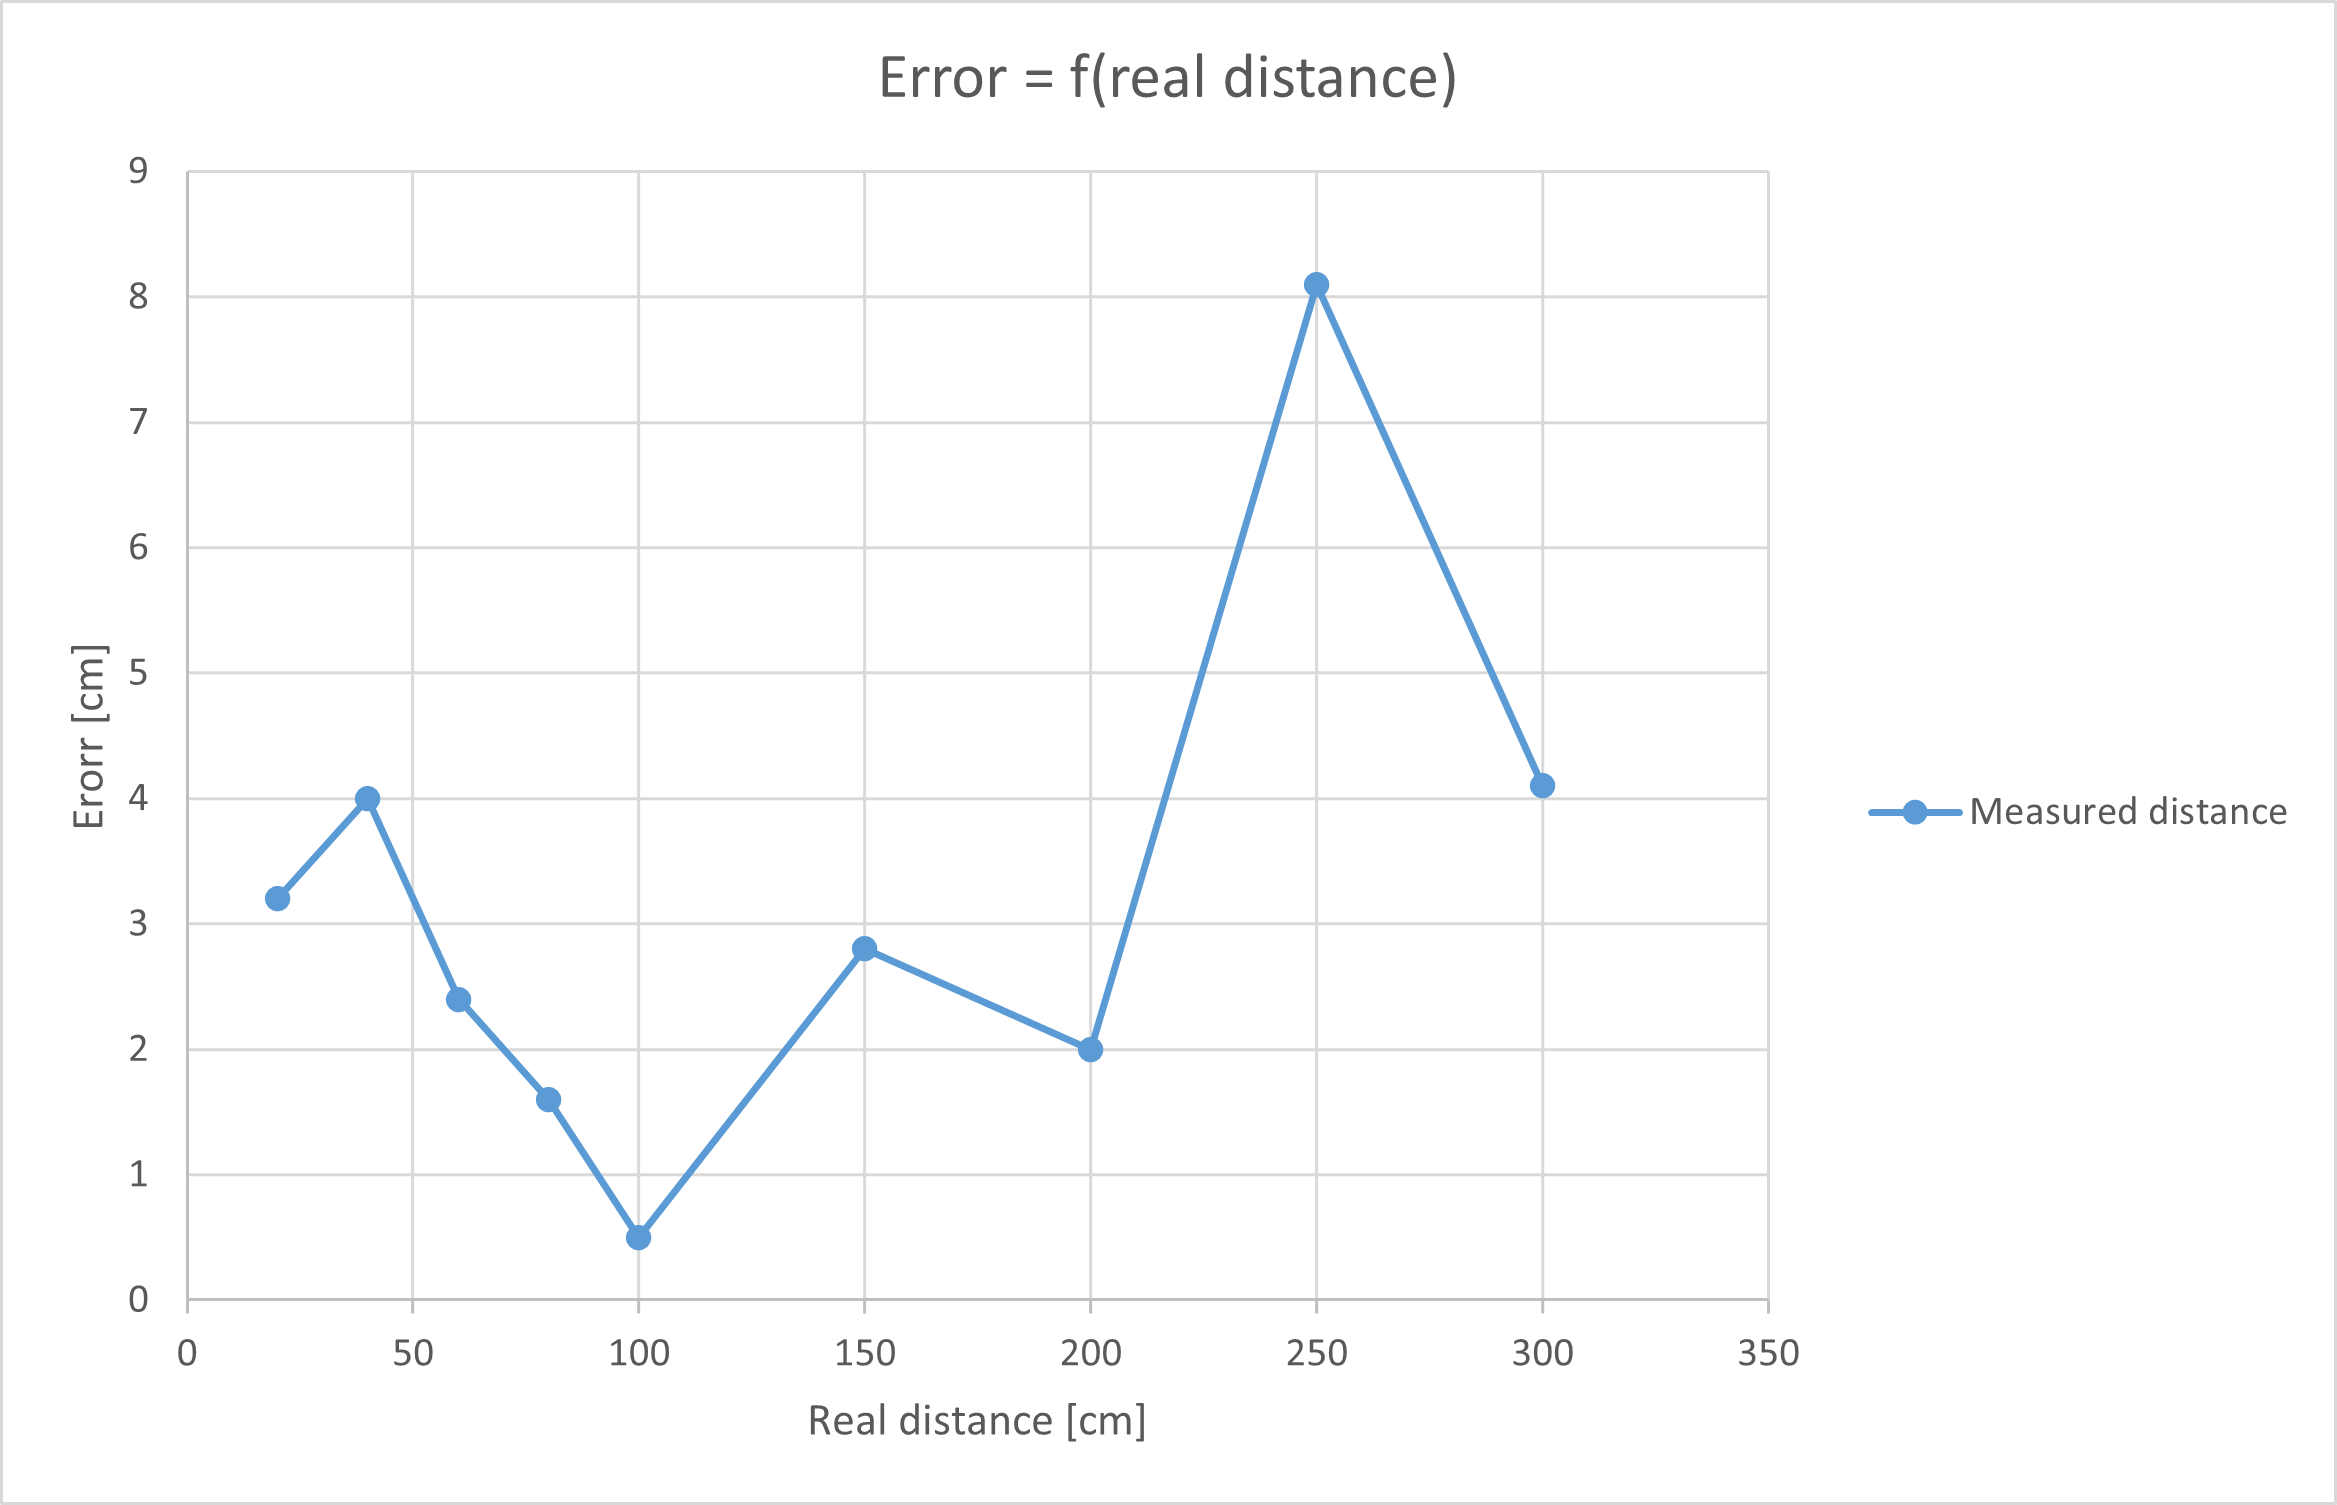
\includegraphics[width=0.8\textwidth]{Images/LiDAR/LiDARRealDistanceGraph_MesDistError_Zoom.png}
    \caption{Erreur de la distance mesurée par rapport à la distance réelle dans la plage utile}
    \label{RealDistanceMesGraphErrorZoom}
\end{figure}

\subsubsection{Conclusion préliminaire}

On constate très facilement sur la figure \ref{RealDistanceMesGraph} que le capteur est perdu au delà
de 3.5m, soit bien moins qu'annoncé par le fabricant. La figure \ref{RealDistanceMesGraphError} nous 
montre une erreur absurde de plus de 5 mètres. On conclut donc que ce capteur ne pourra pas être utilisé
pour des distances de plus de 3.5m.\\
Comme cette grande erreur aplatit totalement les mesures sous 3.5m, nous avons jugé utile d'effectuer un
zoom sur cette plage utile. On constate alors que la distance mesurée par le LiDAR reflète avec plus ou
moins de précision la distance réelle, comme le montre la figure \ref{RealDistanceMesGraphZoom}.
Lorsqu'on trace l'erreur en fonction de la distance réelle, on remarque une erreur généralement bien plus
élevée qu'annoncé (figure \ref{RealDistanceMesGraphErrorZoom}), soit \textpm 1cm pour des distances de 
moins de 2m et \textpm 2cm entre 2 et 4m. Cependant, il faut se rappeler que ce graphe montre uniquement 
l'erreur à la distance réelle, et non l'erreur de répétabilité. Or, comme ces mesures sont un condensé 
de plusieurs séquences espacées dans le temps, on remarque que l'erreur est constante, qui donc peut 
être compensée. De plus, dans le projet, on ne travaille qu'avec des offsets, ce qui limite d'autant 
plus les effets de cette erreur.\par

On peut finalement conclure que ce test est réussi. En effet, malgré une erreur non-négligeable de mesure,
le capteur a une répétabilité constante. Nous pouvons donc passer au test suivant.

\subsection{Mesures de distance dans un environnement perturbé}
\label{MesNoise}

Maintenant que nous savons que le capteur a une répétabilité acceptable, nous cherchons à déterminer comment 
le LiDAR réagit dans un environnement perturbé. Ainsi, un banc de test a été construit afin de projeter 
des confettis devant le capteur lorsqu'il mesure. Les détails de sa construction sont expliqués dans la
section correspondante. Le but final est de générer du bruit de mesure afin de représenter au mieux une
situation réelle, par exemple en pleine tempête de neige. Nous pourrons ainsi développer une méthode
de mesure qui permet en tout temps de mesurer une hauteur de neige.

\subsubsection{Méthode}

Afin de vérifier ce test, le capteur ainsi que la plaque de développement ont été montés sur un trépied
à environ 1.5m au-dessus du sol, avec un angle de 60° par rapport à la verticale. Le LiDAR pointe le sol,
nettoyé au préalable et donc sans confetti. 100 mesures de distance sont réalisées à chaque série afin
d'avoir assez d'échantillons pour quantifier le bruit généré.\\
Sur l'appui du bouton utilisateur de la carte, le programme lance une série de 100 mesures en direction
du sol. Cela nous permet dans un premier temps d'avoir une distance de référence à comparer, sans aucune
perturbation. \\
Ensuite, quatre autres séries de mesures sont effectuées, avec quatre niveaux arbitraires de perturbation
différents, générés manuellement par les opérateurs, comme le montre la figure \ref{ErrorMesSetup}.

\begin{figure}[H]
    \centering
    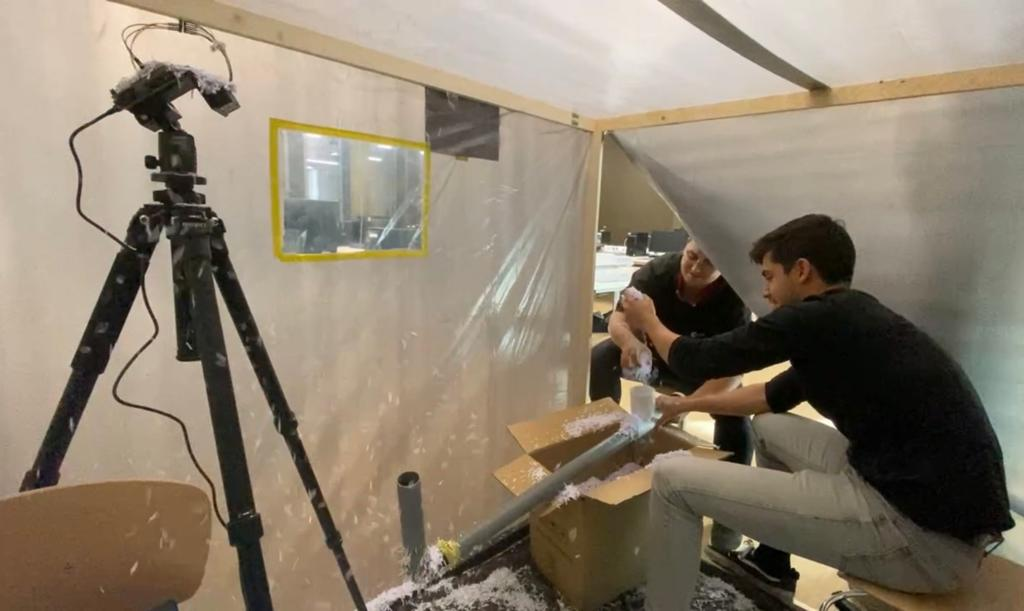
\includegraphics[width=0.75\textwidth]{Images/LiDAR/ErrorMesSetup.jpeg}
    \caption{Mise en place du test de perturbation}
    \label{ErrorMesSetup}
\end{figure}

\subsubsection{Résultats du test}

\begin{figure}[H]
    \centering
    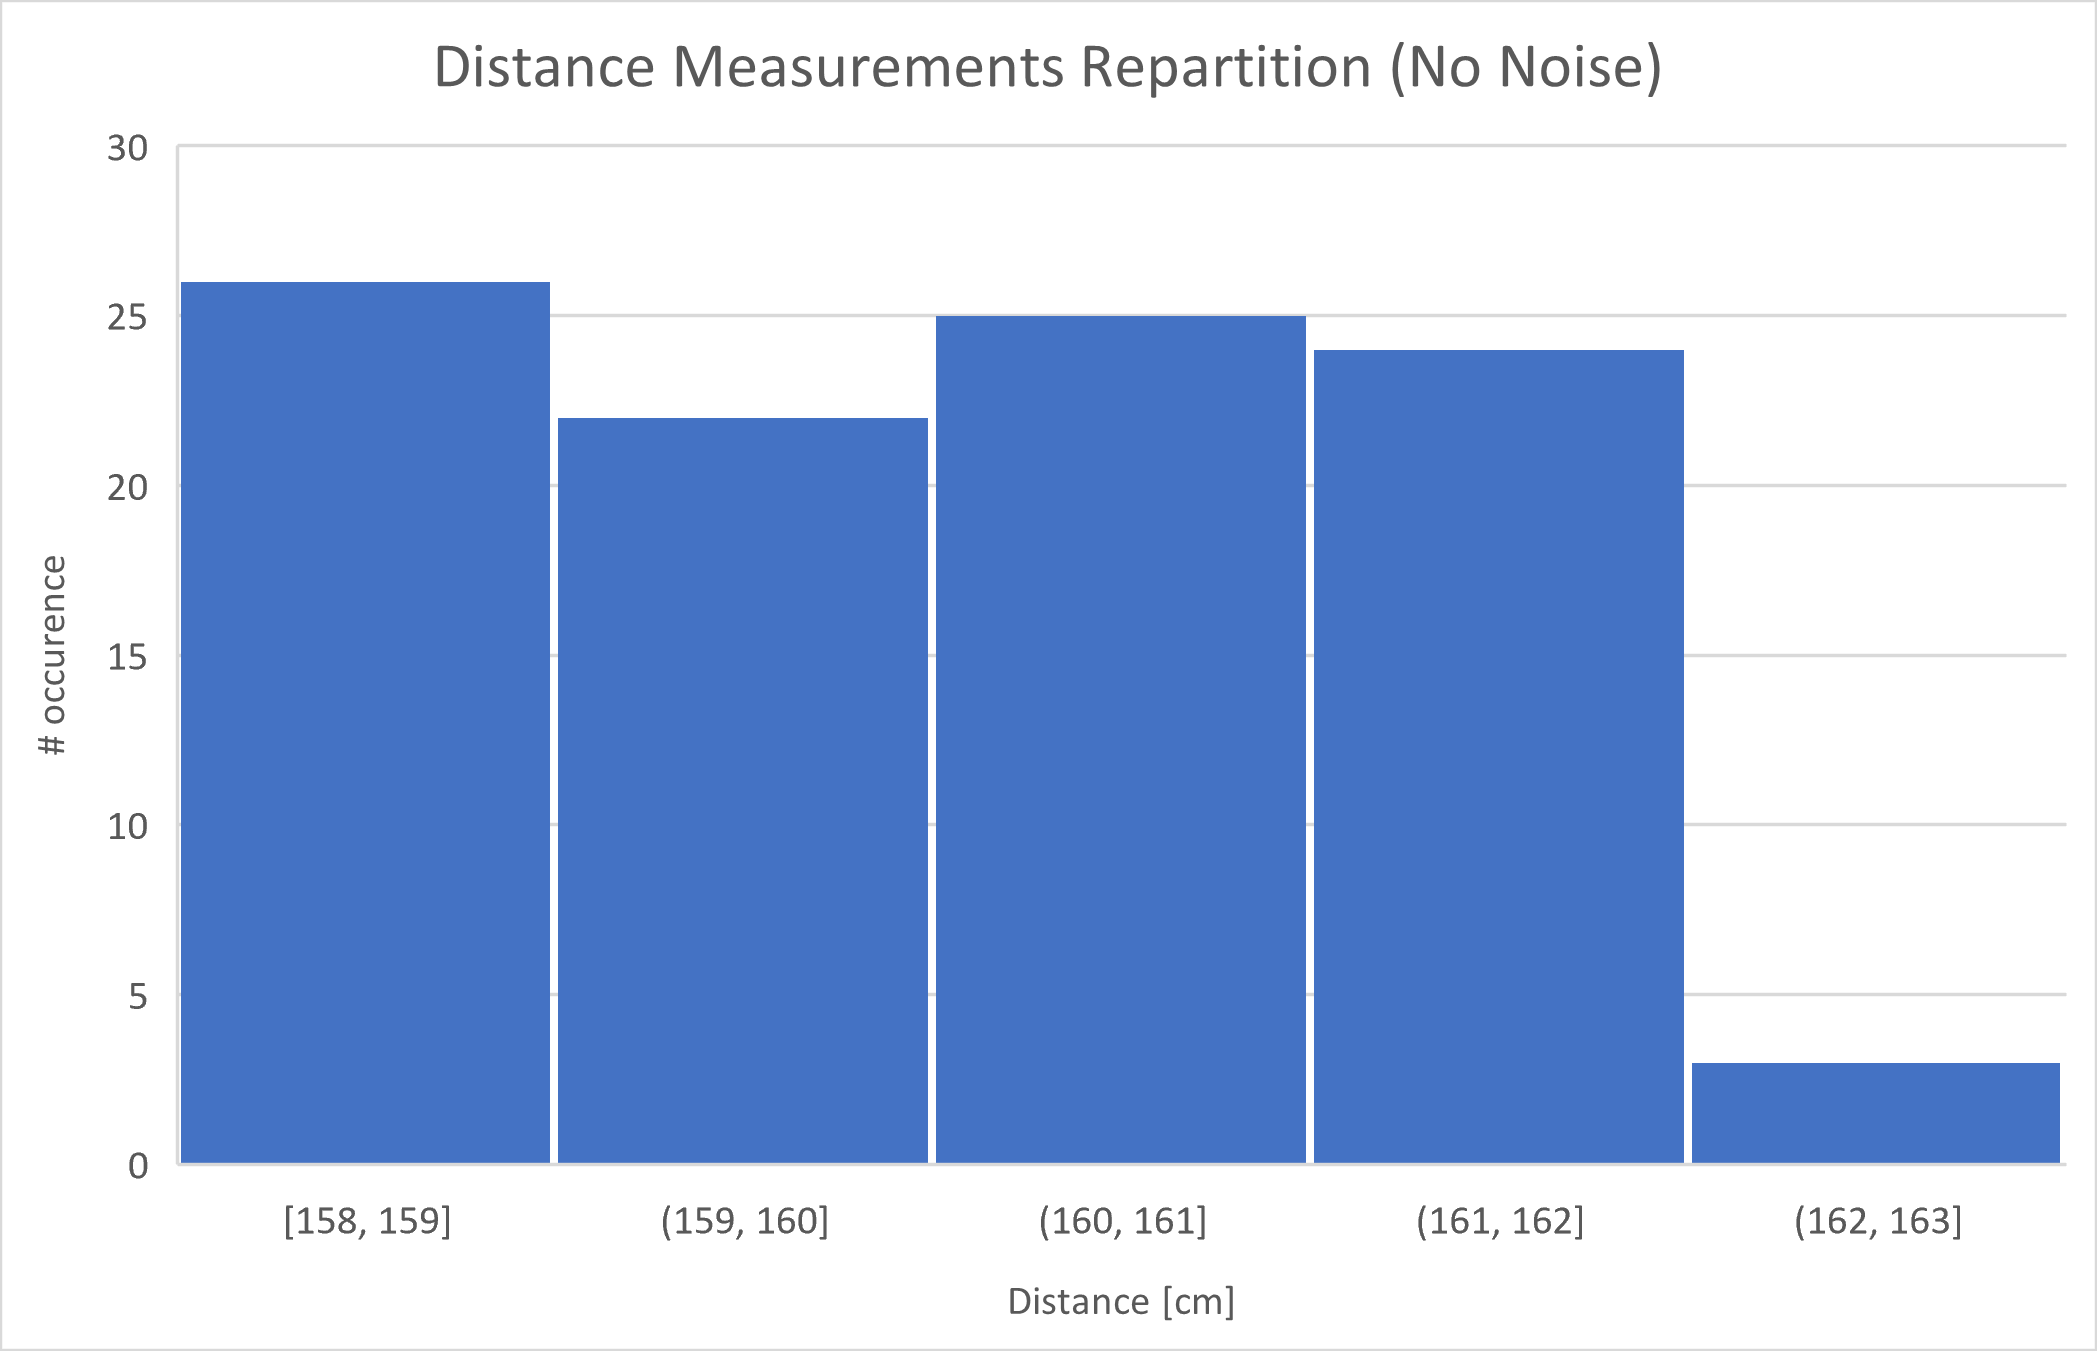
\includegraphics[width=0.8\textwidth]{Images/LiDAR/LiDAR_ErrorMes_NoNoise.png}
    \caption{Histogramme de la mesure de référence}
    \label{ErrorMesRefDist}
\end{figure}

\begin{figure}[H]
    \centering
    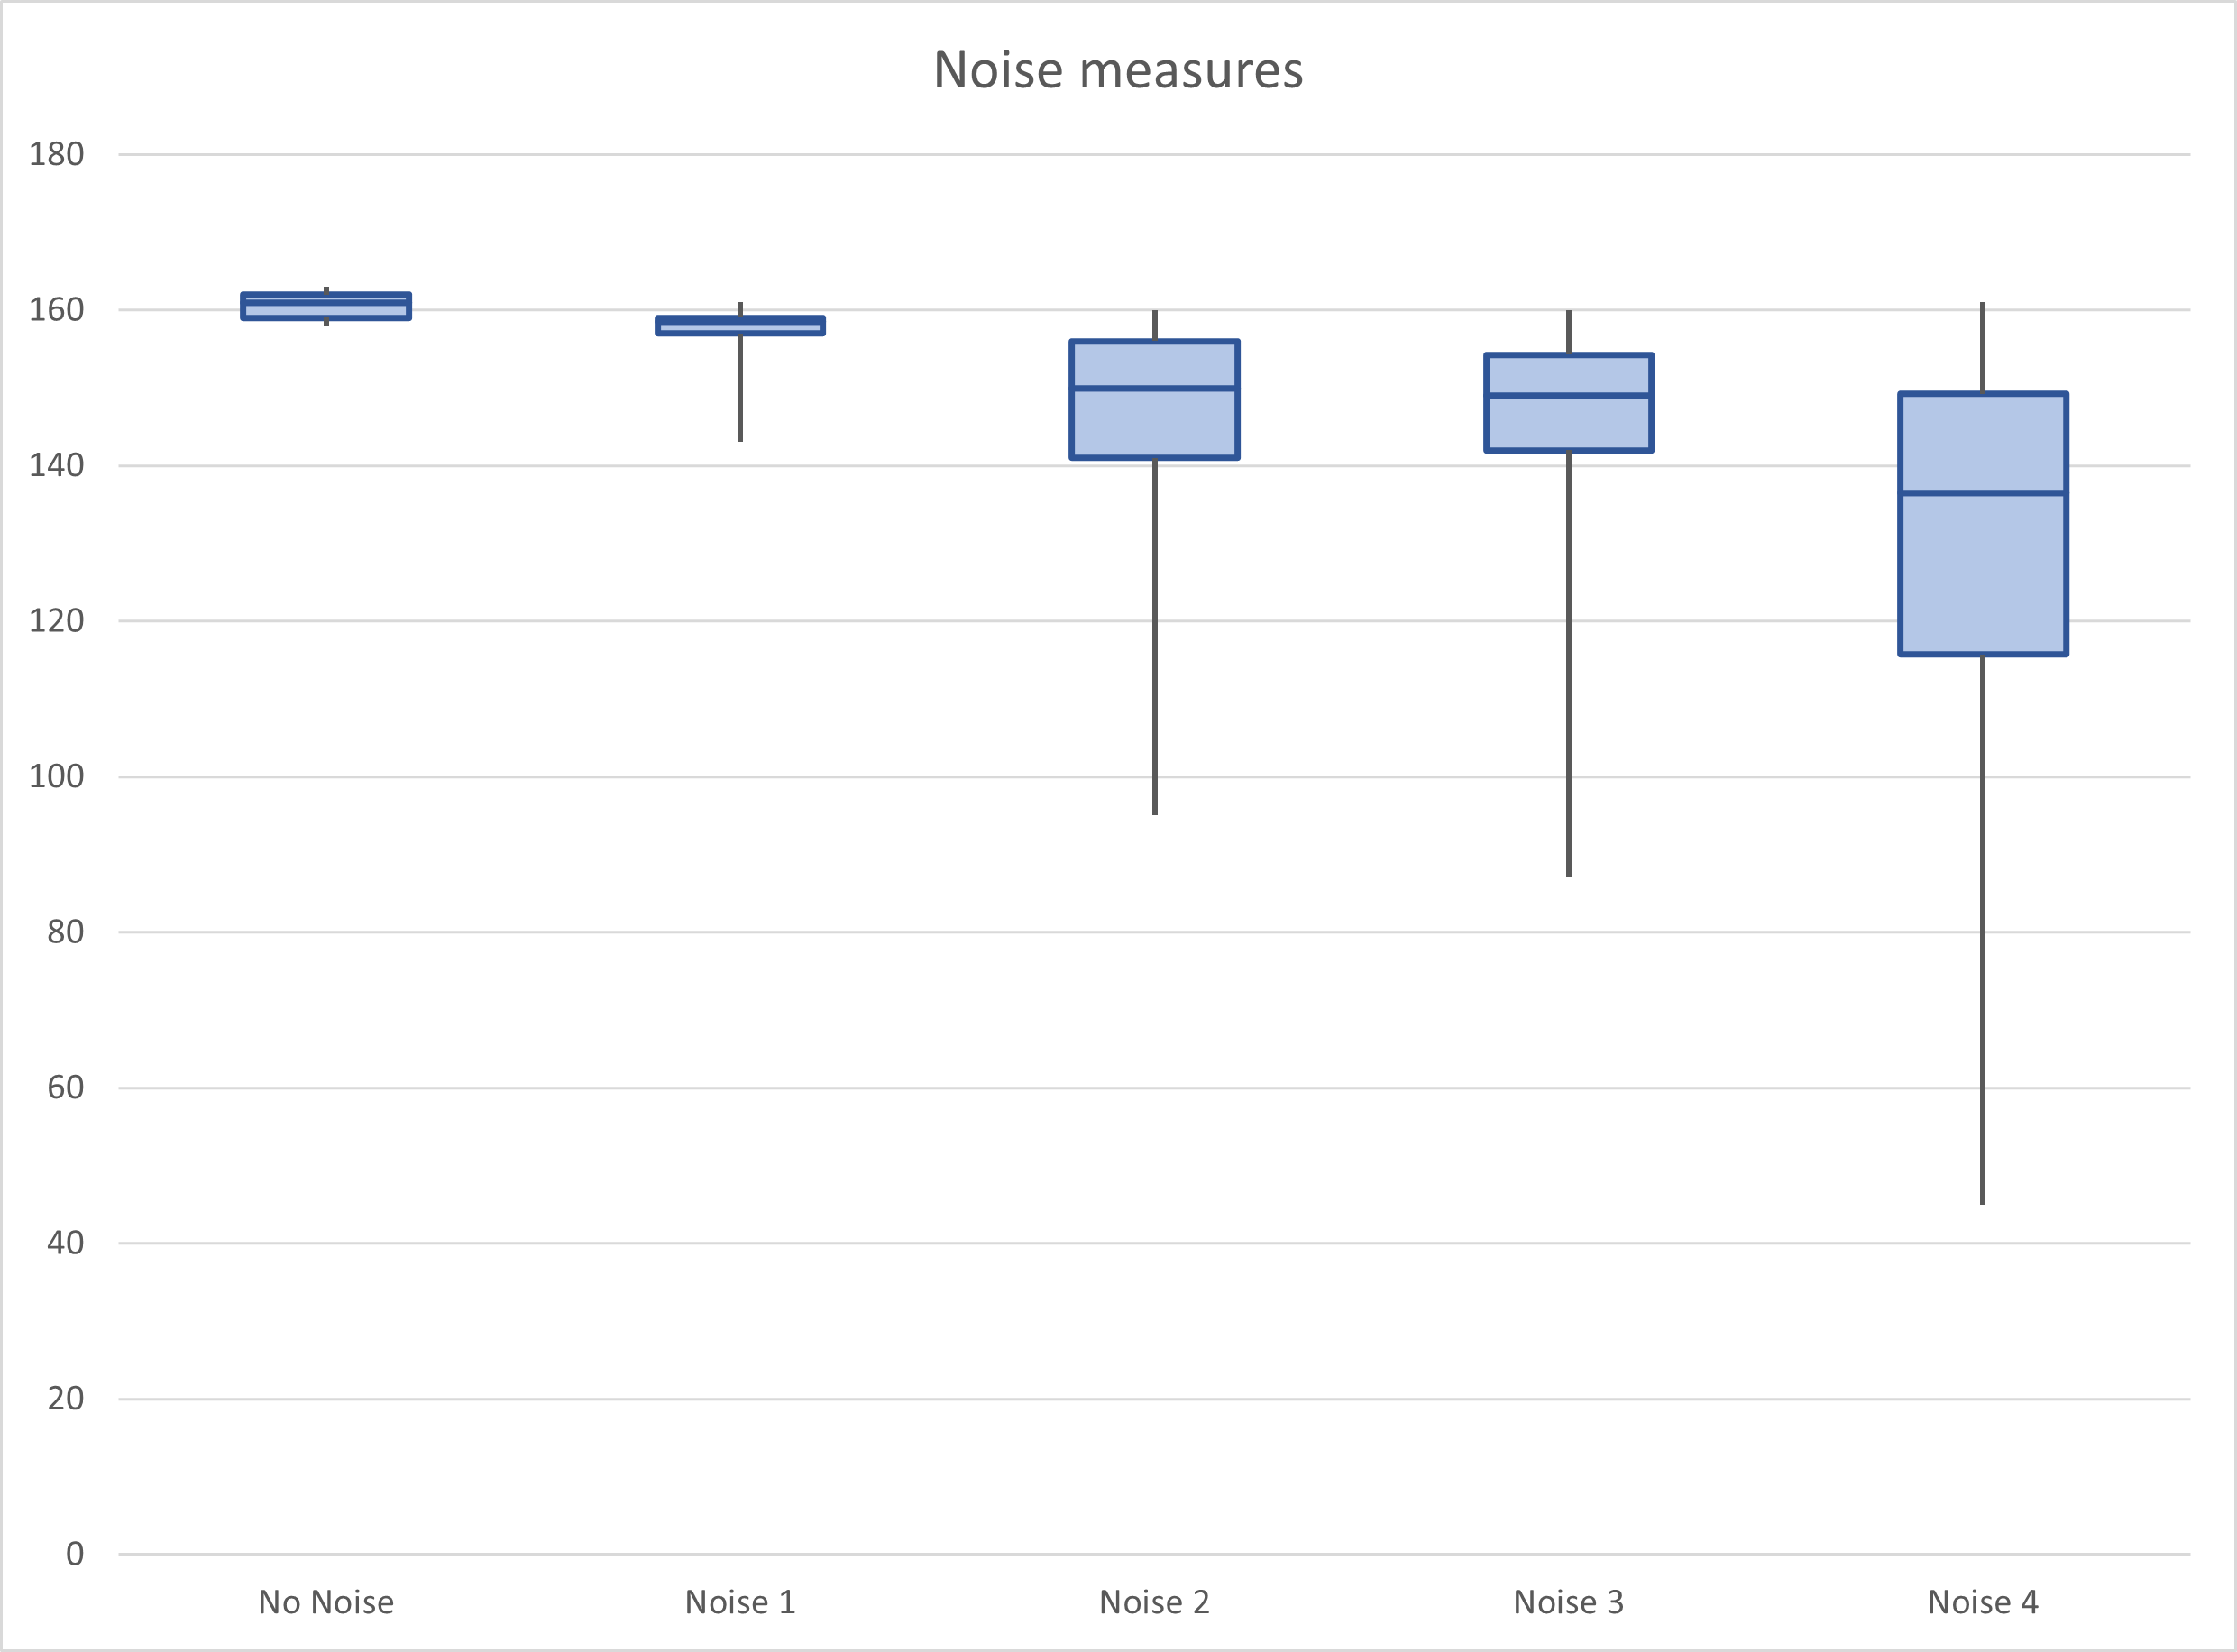
\includegraphics[width=0.8\textwidth]{Images/LiDAR/LiDAR_ErrorMes_Moustache.png}
    \caption{Comparaison des 5 mesures effectuées}
    \label{ErrorMesMoustache}
\end{figure}

Les 5 mesures ont été regroupées en un seul graphe de type "Boîte à moustaches" afin de pouvoir
comparer avec plus d'aisance les mesures entre-elles. De gauche à droite, on retrouve une augmentation
graduelle du bruit généré par les opérateurs.

\begin{table}[H]
    \centering
    \begin{tabular}{|c|c|c|c|c|c|}
        \hline
        & No Noise & Noise 1 & Noise 2 & Noise 3 & Noise 4 \\
        \hline\hline
        Mean & 160.52 & 157.77 & 145.44 & 145.06 & 127.78 \\
        \hline
        Median & 161 & 158.8 & 150 & 149 & 136.5 \\
        \hline
        Max & 163 & 161 & 160 & 160 & 161 \\
        \hline
        
    \end{tabular}
    \caption{Différentes méthodes de calcul de distance (en cm)}
    \label{ComputingMethods}
\end{table}

Afin d'avoir la méthode la plus représentative possible de la distance au sol, trois solutions 
ont été envisagées. À partir de la série de mesures, nous avons calculé la moyenne, la médiane
ainsi que le maximum afin de déterminer laquelle de ces valeurs représente le plus la réalité.\\
//ANNEXE A : HISTOGRAMME DE CHACUNE DES MESURES

\subsubsection{Conclusion préliminaire} 

Premièrement, la figure \ref{ErrorMesRefDist} montre l'histogramme des 100 mesures de référence au sol.
Elles s'avèrent plutôt rassurantes car on remarque que la répétabilité des mesures est respectée, avec
une précision typique de \textpm 2cm. La plupart des mesures sont réparties uniformément autour de 160cm.\par
On distingue ensuite sur la figure \ref{ErrorMesMoustache} que le bruit de mesure a bel et bien augmenté
au fil des séries, représenté par la longueur des barres d'erreur. Comme l'indique le principe des boîtes
à moustache, le trait central du rectangle représente la médiane des valeurs, alors que les deux autres
sont le premier et troisième quartiles. Ainsi, les valeurs médianes des séries s'éloignent de plus en 
plus de la distance au sol (de référence).\par
Le but final de la figure \ref{ErrorMesMoustache} est d'aider à déterminer quelle est la méthode
de mesure la plus efficace pour calculer des distances dans un environnement perturbé. On remarque
ainsi d'ores et déjà que la médiane n'est pas un outil fiable, puisque sa valeur d'éloigne de plus en
plus de la référence au fil des séries. Cependant, on voit facilement que les valeurs maximales de chaque
boîte s'approche très fortement de la distance de référence.\\
La table \ref{ComputingMethods} nous aide à y voir plus clair en ce qui concerne l'efficacité de ces
trois méthodes. Pour rappel, selon la mesure de référence, la distance au sol à mesurer est de 160cm.

\begin{description}
    \item[Moyenne] La moyenne représente la meilleure méthode dans le cas d'une mesure sans aucune 
    perturbation. Cependant, on voit que cette méthode devient très imprécise lorsque du bruit
    apparaît devant le capteur.
    \item[Médiane] Malgré le fait que la médiane soit généralement plus proche de la réalité par rapport 
    à la moyenne, elle est encore beaucoup trop éloignée de la vraie distance au sol. L'erreur est à 
    nouveau de plus en plus grande dès que les perturbations augmentent. 
    \item[Maximum] La méthode du maximum semble donner une valeur très proche de la vraie distance,
    et ce peu importe le niveau de perturbation devant le capteur. Il suffit en effet qu'une valeur
    de la série soit la mesure du sol pour que cette méthode fonctionne. Nous comptons donc sur le fait 
    que, statistiquement, on finisse toujours par faire au moins une mesure de la distance au sol dans 
    la série.
\end{description}

Il semblerait que pour le moment, la méthode du maximum obtienne les résultats les plus prometteurs.
Cependant, nous garderons ces 3 méthodes pour les tests suivants afin de confirmer ou non l'efficacité
des techniques de calcul.

\subsection{Stabilité en température des mesures}

Le capteur, intégré dans un boîtier étanche, sera soumis à des températures qui varient constamment,
de -20°C lors d'une nuit glaciale jusqu'à 30 voire 40°C à l'intérieur du boîtier, en plein soleil.
Il est important de savoir comment les mesures prises par le LiDAR vont être influencées par cette 
variation.\\
À titre d'exemple, imaginons que le système prenne une mesure de distance de référence afin d'être
prêt à mesurer des hauteurs de neige. Le soleil vient de se coucher, mais une température de 15°C
reigne encore dans le boîtier. Plus tard dans la nuit, alors qu'il fait -5°C, il commence à neiger.
Le système de détection se met en marche et commence à mesurer des offsets. Ces derniers seront
peut-être faussés par une différence de 20°C entre la mesure de référence et la mesure actuelle !

\subsubsection{Méthode}

Le LiDAR et la plaque de développement sont fixés sur un trépied et sont placés dans une chambre
climatique (de la marque \emph{Vötsch}, modèle 4010) afin de faire varier la température ambiante.
Comme décrit dans le paragraphe ci-dessus, le système sera soumis à des températures entre -20°C et
40°C. C'est pour cela que le capteur sera soumis à cette même plage de températures, par pas de 5°C.\\
La distance entre le capteur et la paroi opposée de la chambre climatique est de 47cm. Les mesures 
sont récupérées via le port COM qui lie la carte à l'ordinateur. La figure \ref{TempError} montre 
la mise en place du test, avec le capteur à l'intérieur de la chambre.

\begin{figure}[H]
    \centering
    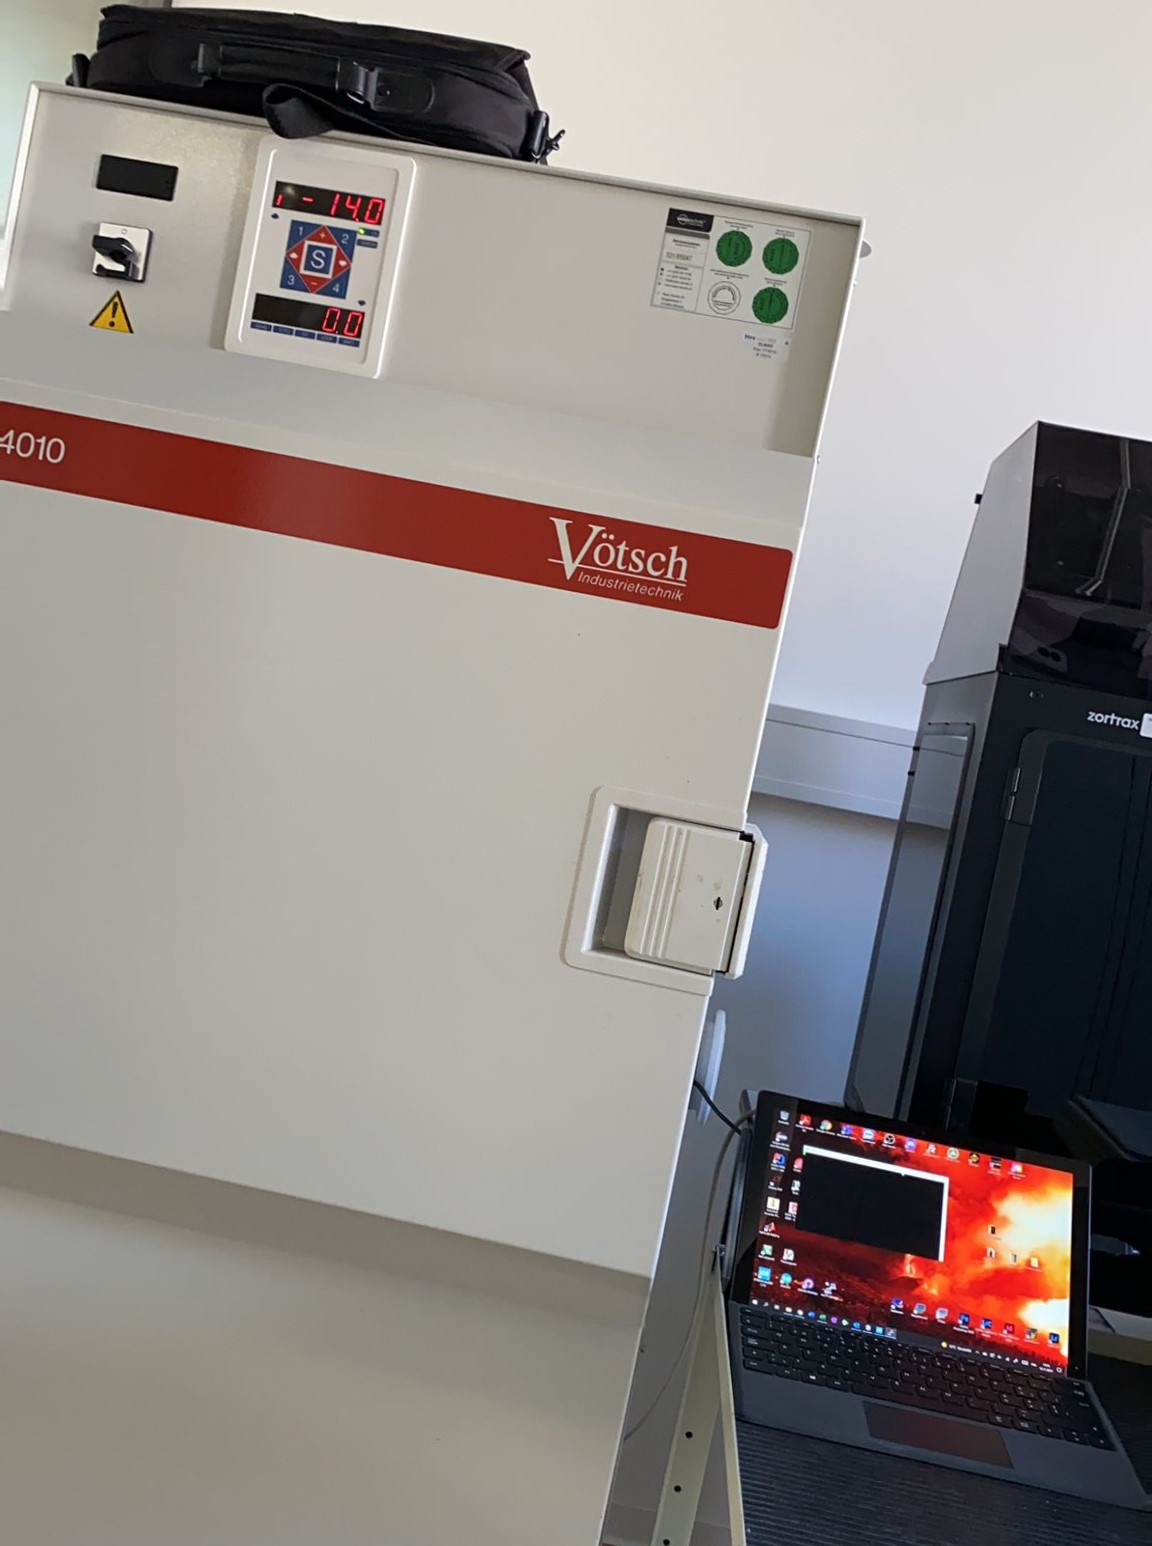
\includegraphics[width=0.5\textwidth]{Images/LiDAR/TempMes.jpeg}
    \caption{Mise en place du test en température}
    \label{TempError}
\end{figure}

\subsubsection{Résultats du test}

\begin{figure}[H]
    \centering
    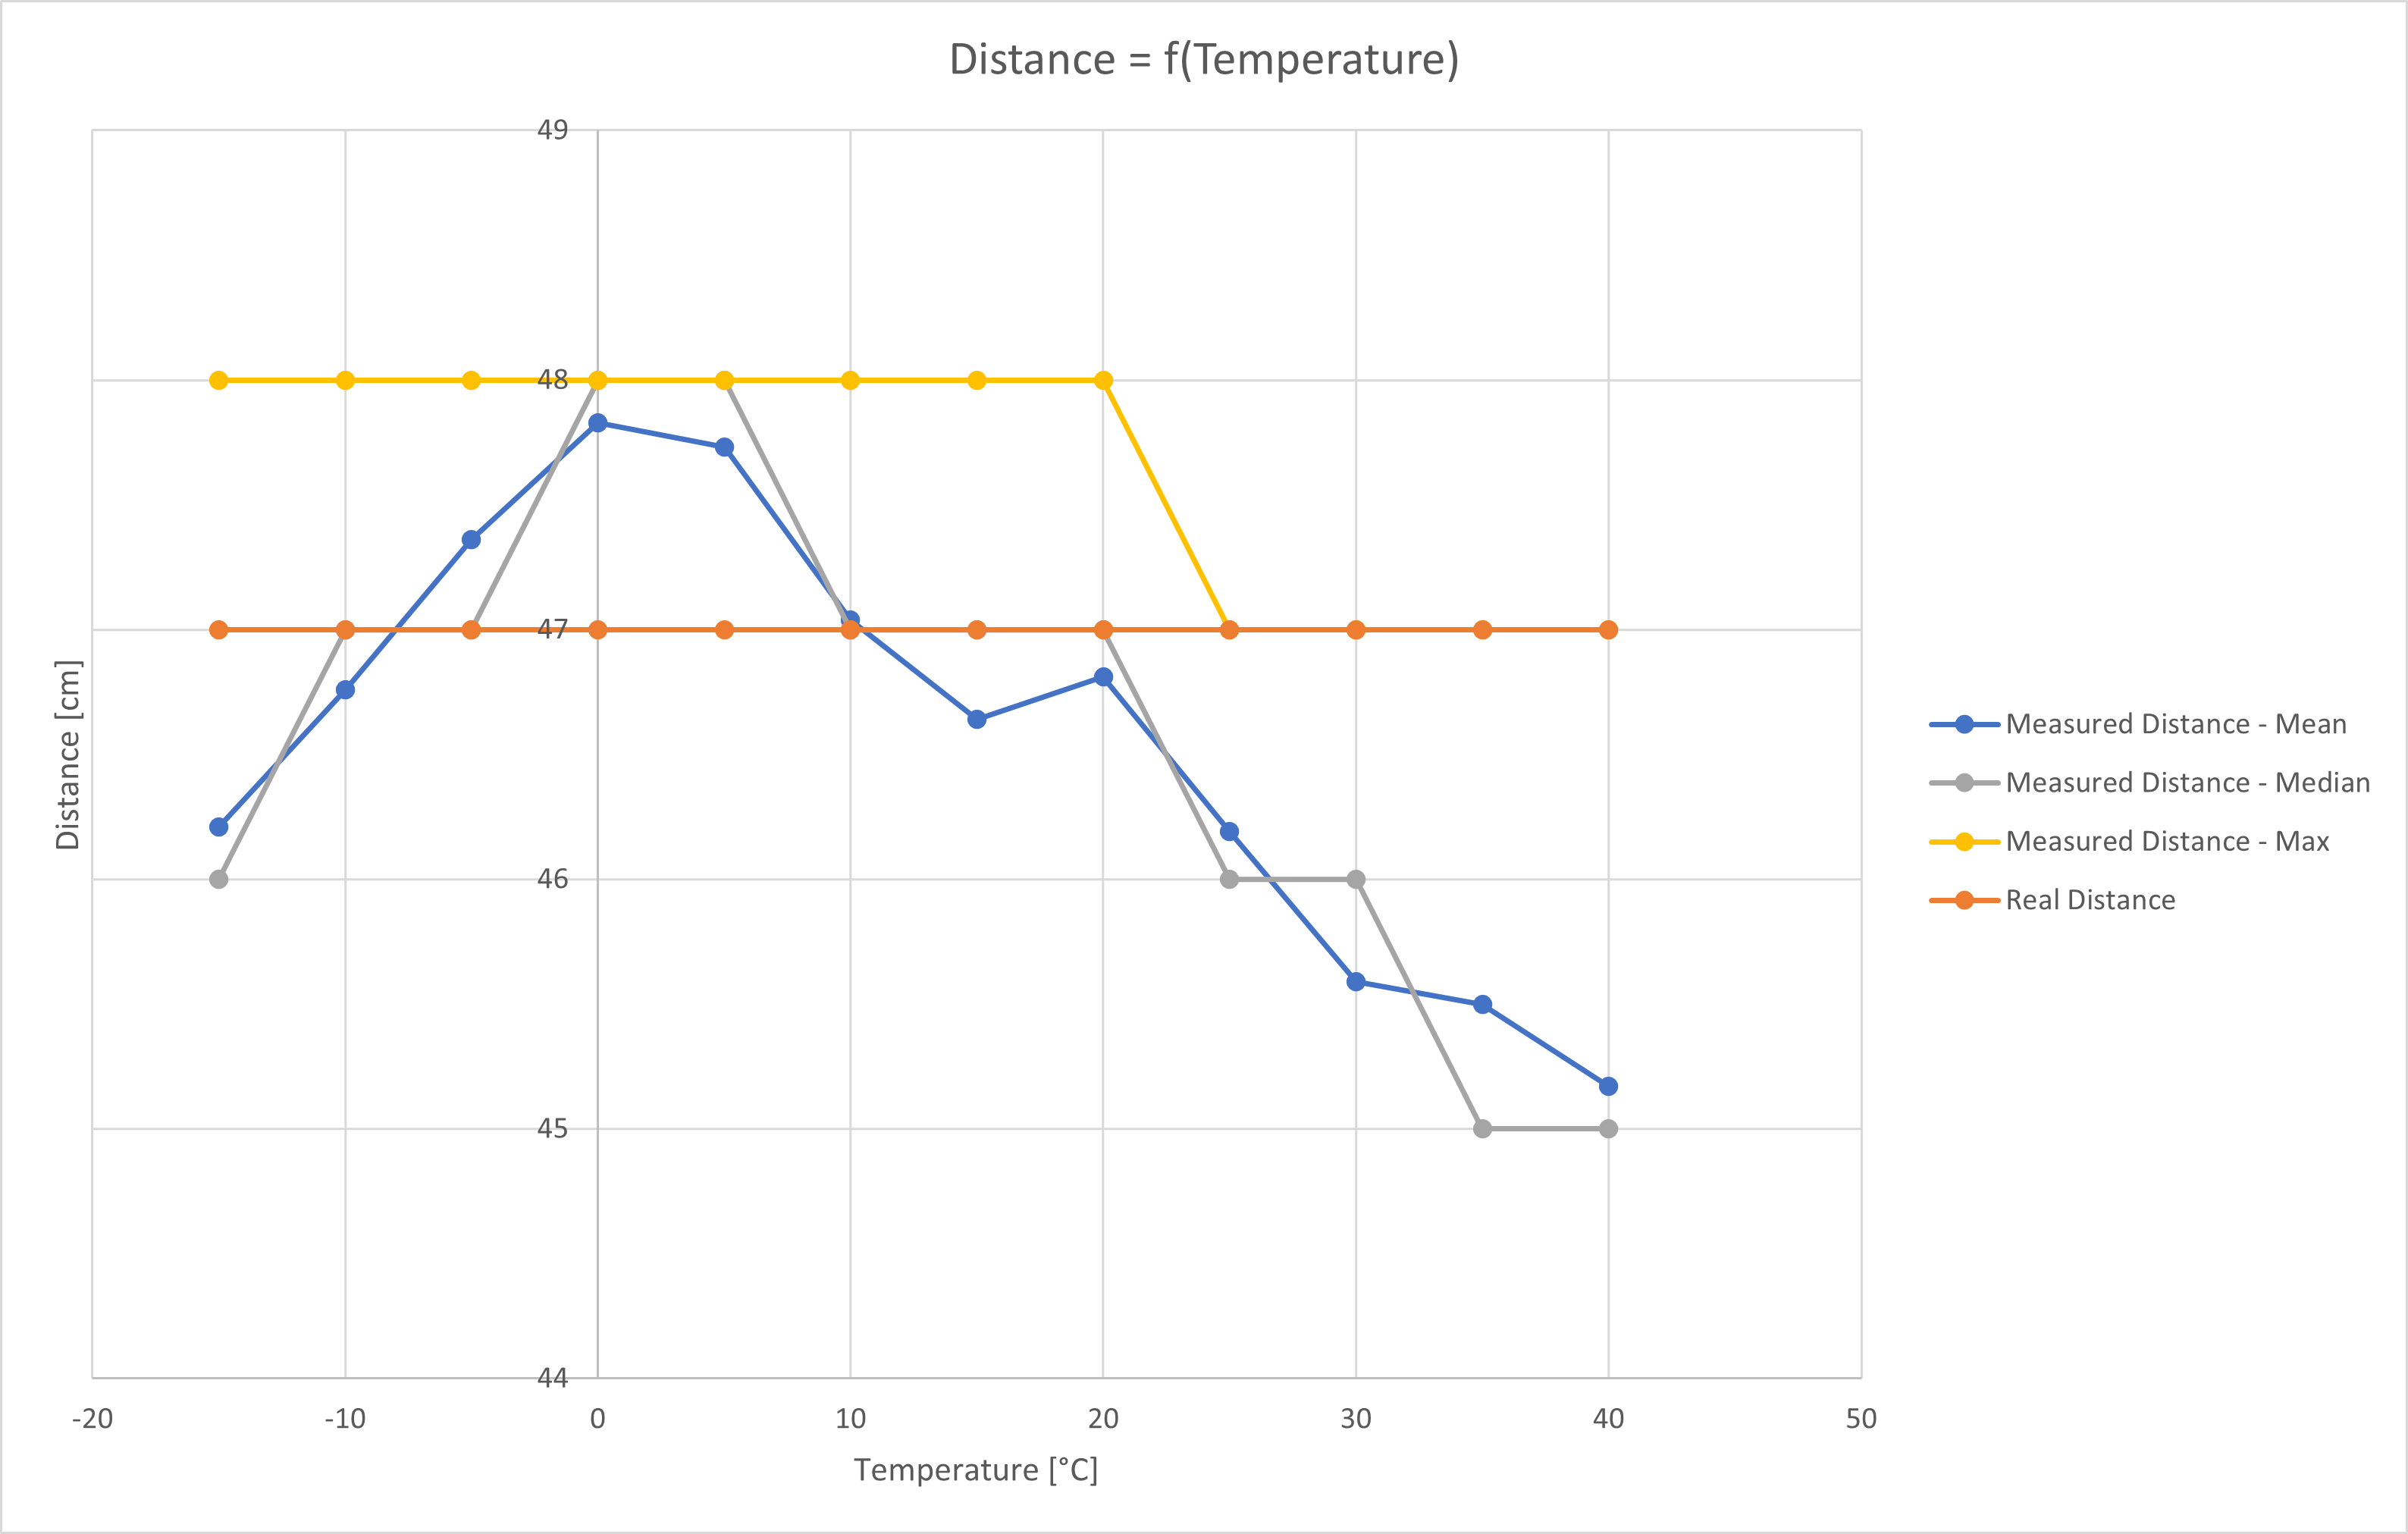
\includegraphics[width=0.8\textwidth]{Images/LiDAR/LiDAR_TempStabilityGraph.png}
    \caption{Graphe de stabilité en température du LiDAR}
    \label{TempErrorGraph}
\end{figure}

Le test a été réalisé à partir d'une température de -15°C et non pas de -20°C. En effet, la chambre
climatique utilisée n'était pas en mesure d'atteindre cette consigne dans un temps raisonnable.\\
Les trois méthodes décrites dans le test précédent ont été reprises afin de mieux comprendre la
répartition des valeurs mesurées.

\subsubsection{Conclusion préliminaire} 

Il semblerait que le capteur soit relativement peu influencé par la variation de température. En
effet, en plus de sa résolution fixe de 1cm, nous avons une erreur typique de \textpm 2cm autour
de la valeur réelle.\\
Cependant, on constate tout de même que la moyenne et la médiane sont plus influencées que la méthode
du maximum. On peut ainsi conclure que le capteur est plutôt stable en température, surtout si on
utilise le maximum comme méthode de mesure.\par 
On peut considérer finalement que le capteur est fiable pour une mesure de référence et de hauteur
de neige prises à des températures différentes, comme cette différence est noyée dans sa précision
typique.

\subsection{Mesure de hauteur en laboratoire}

Maintenant que nous avons caractérisé ce capteur pour plusieurs situations, nous pouvons procéder aux
véritables mesures d'épaisseur en laboratoire. En effet, il faut à présent vérifier si la méthode de
calcul de la section \ref{MethodeDeMesure} est réalisable en condition de laboratoire dans un premier
temps.

\subsubsection{Méthode}

Pour effectuer ce test, le capteur est placé dans le banc de test à une hauteur $h$ de 133cm au-dessus
du sol. L'angle $\alpha$ du LiDAR a été fixé à 60°, alors que l'angle $\beta$ est de 0°. Ces informations 
ont été fournies au programme de test afin de calculer des bons offsets. La figure \ref{OffsetMes_Labo}
montre la préparation au test.\\
Le but est de mesurer tout d'abord une distance de référence au sol, sans aucun obstacle ni bruit de
mesure. Ensuite, une fois la plaque placée, on effectue quatre mesures différentes, la première sans
bruit puis avec un bruit graduel généré par les opérateurs.\\
L'obstacle utilisé est une plaque en mousse blanche de protection, d'une épaisseur de 6.6cm.

\begin{figure}[H]
    \centering
    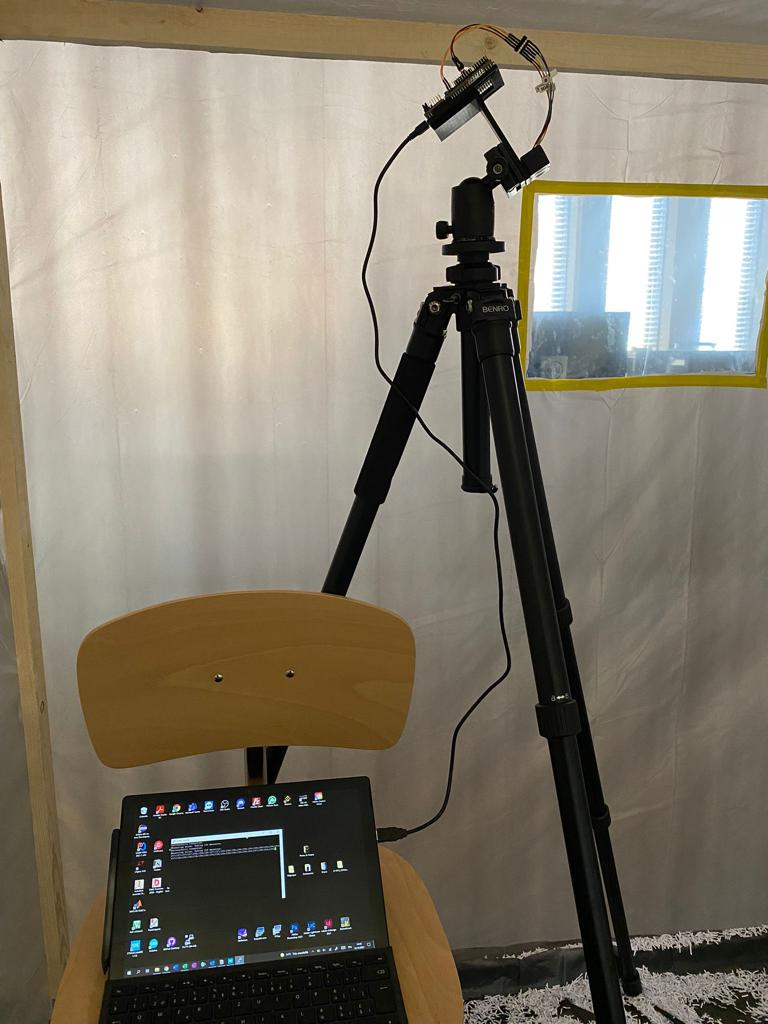
\includegraphics[width=0.5\textwidth]{Images/LiDAR/OffsetMes_InLab.jpeg}
    \caption{Mise en place du test de mesure d'épaisseur}
    \label{OffsetMes_Labo}
\end{figure}

\subsubsection{Résultats du test}

\begin{figure}[H]
    \centering
    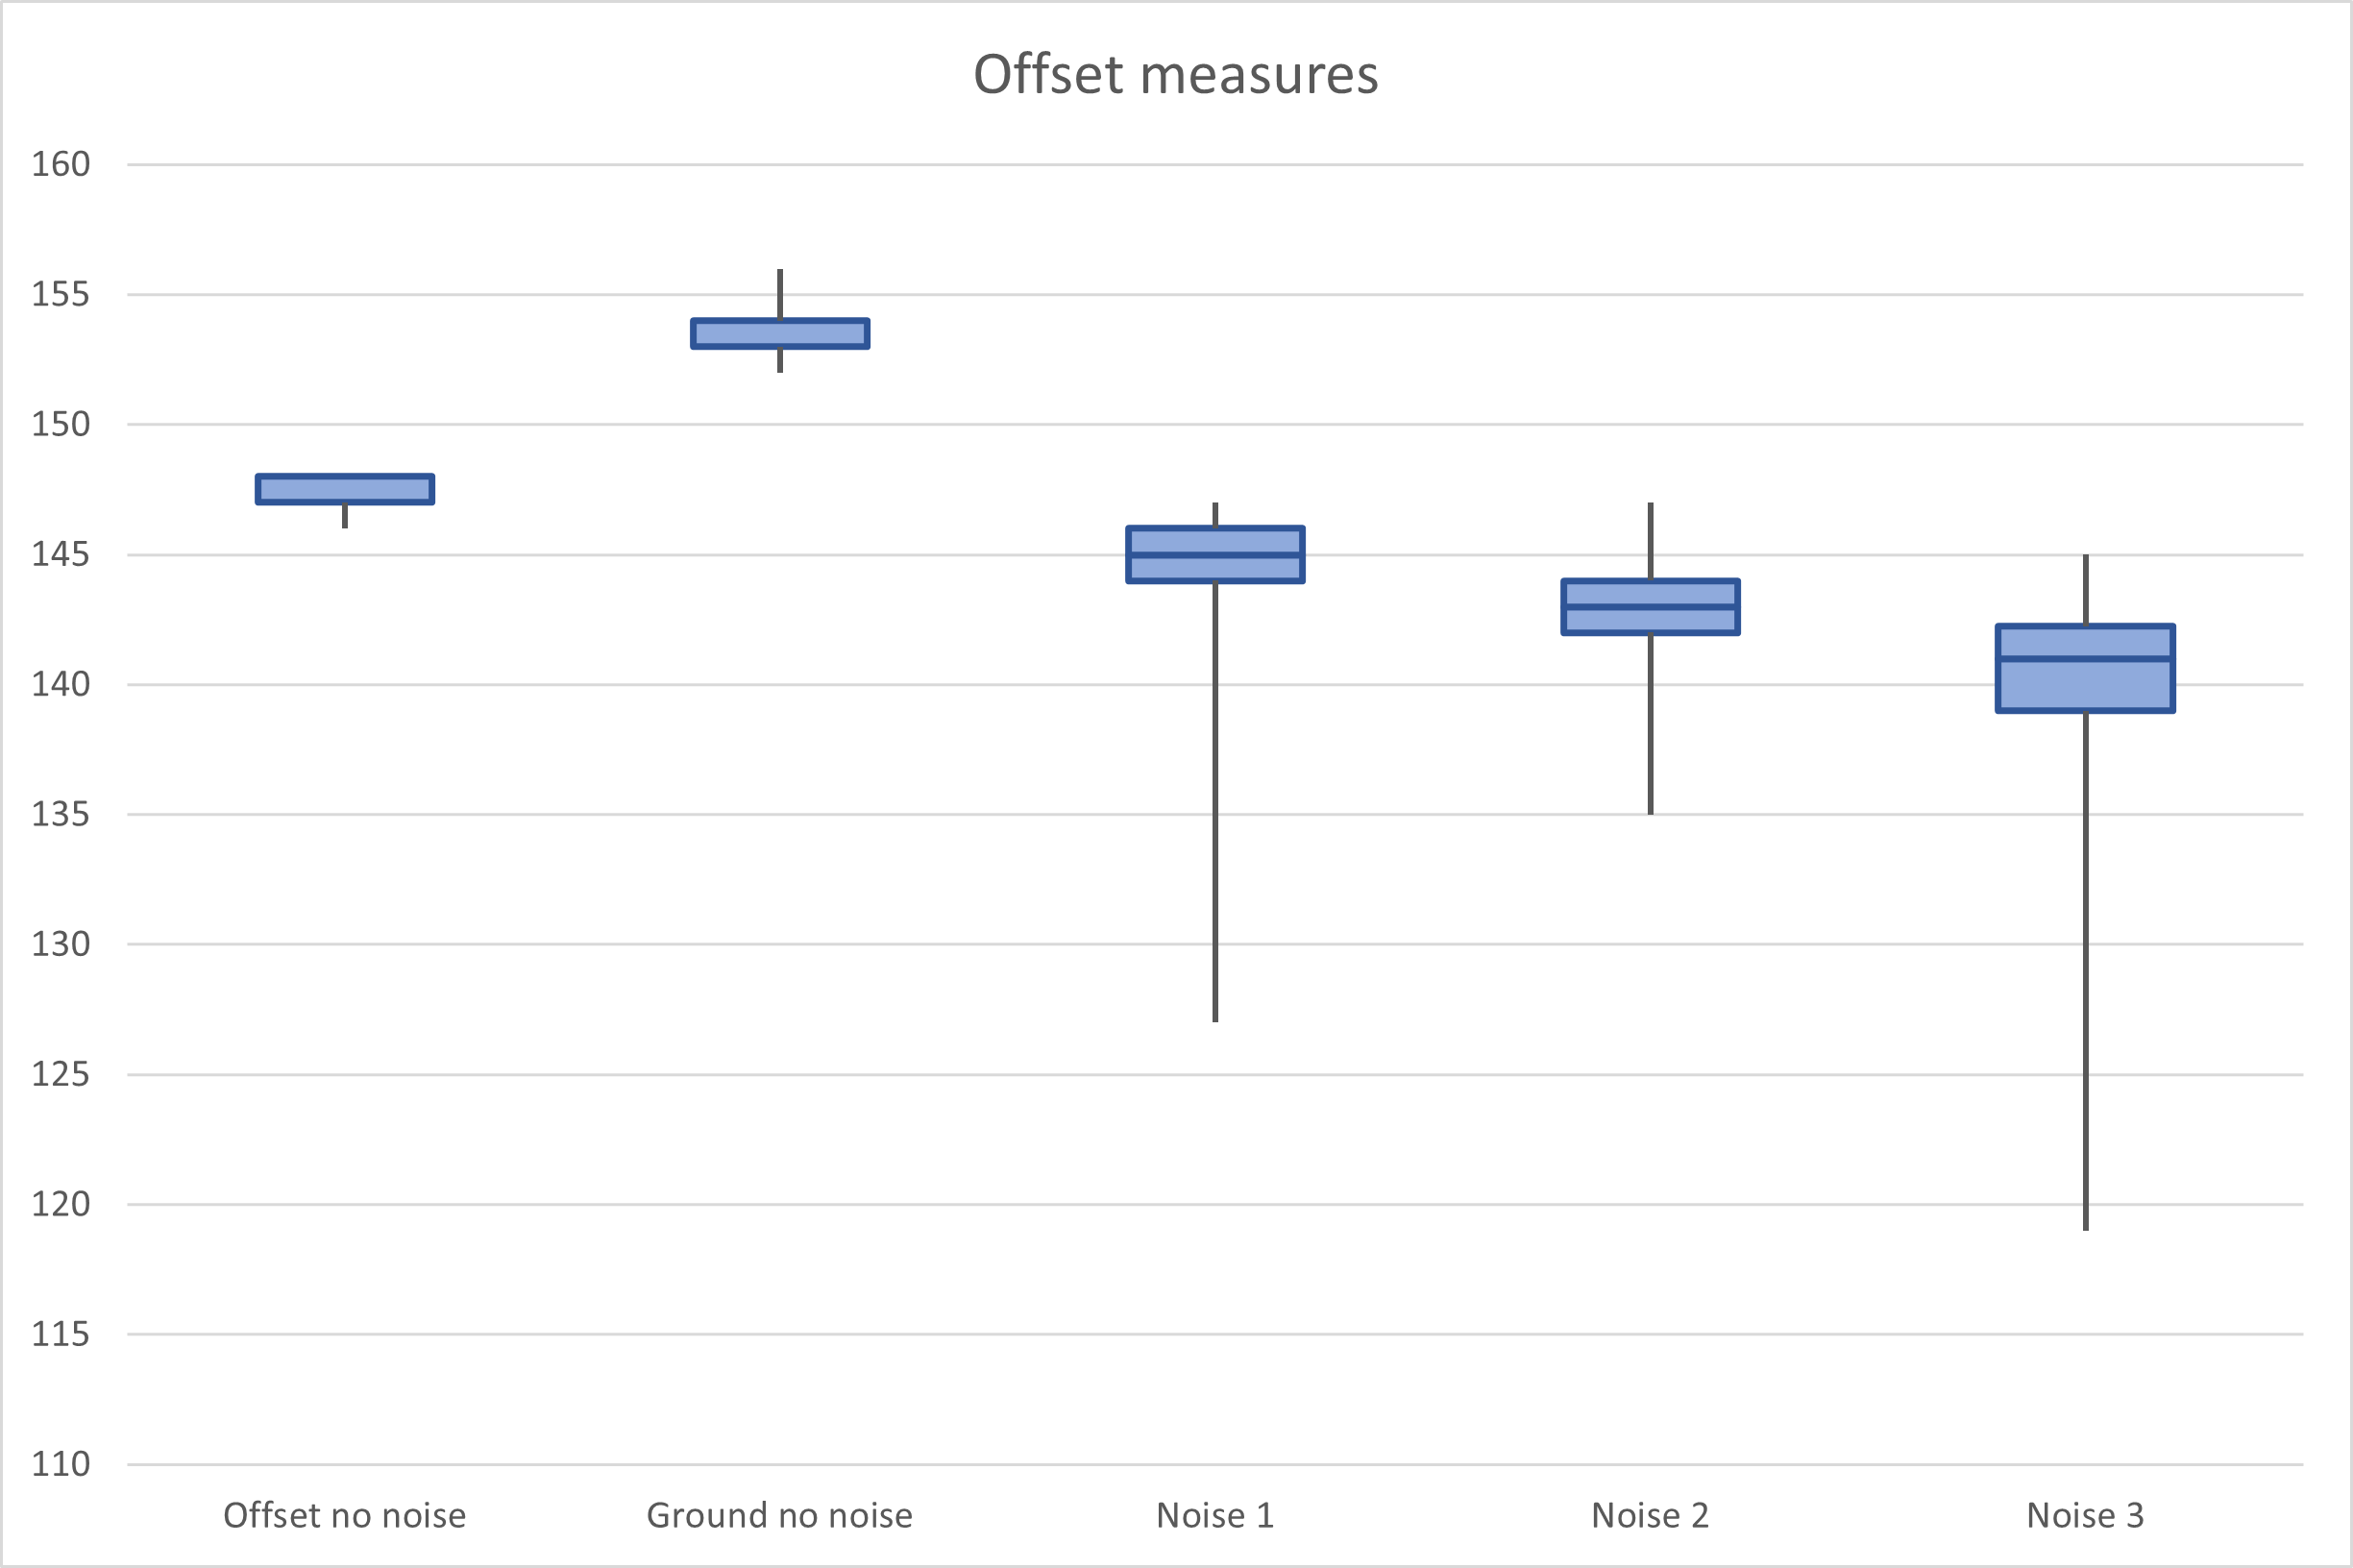
\includegraphics[width=0.8\textwidth]{Images/LiDAR/LiDAR_OffsetMes_Moustache.png}
    \caption{Boîte à moustache des mesures d'épaisseur}
    \label{OffsetMes_Moustache}
\end{figure}

Il est important de noter que pour la série de mesure \emph{Noise 3}, la valeur maximale n'atteint
pas celle des autres séries. Cela est dû majoritairement au fait qu'une couche de 2cm de confettis
se sont accumulés sur la plaque au fil des mesures.

\begin{figure}[H]
    \centering
    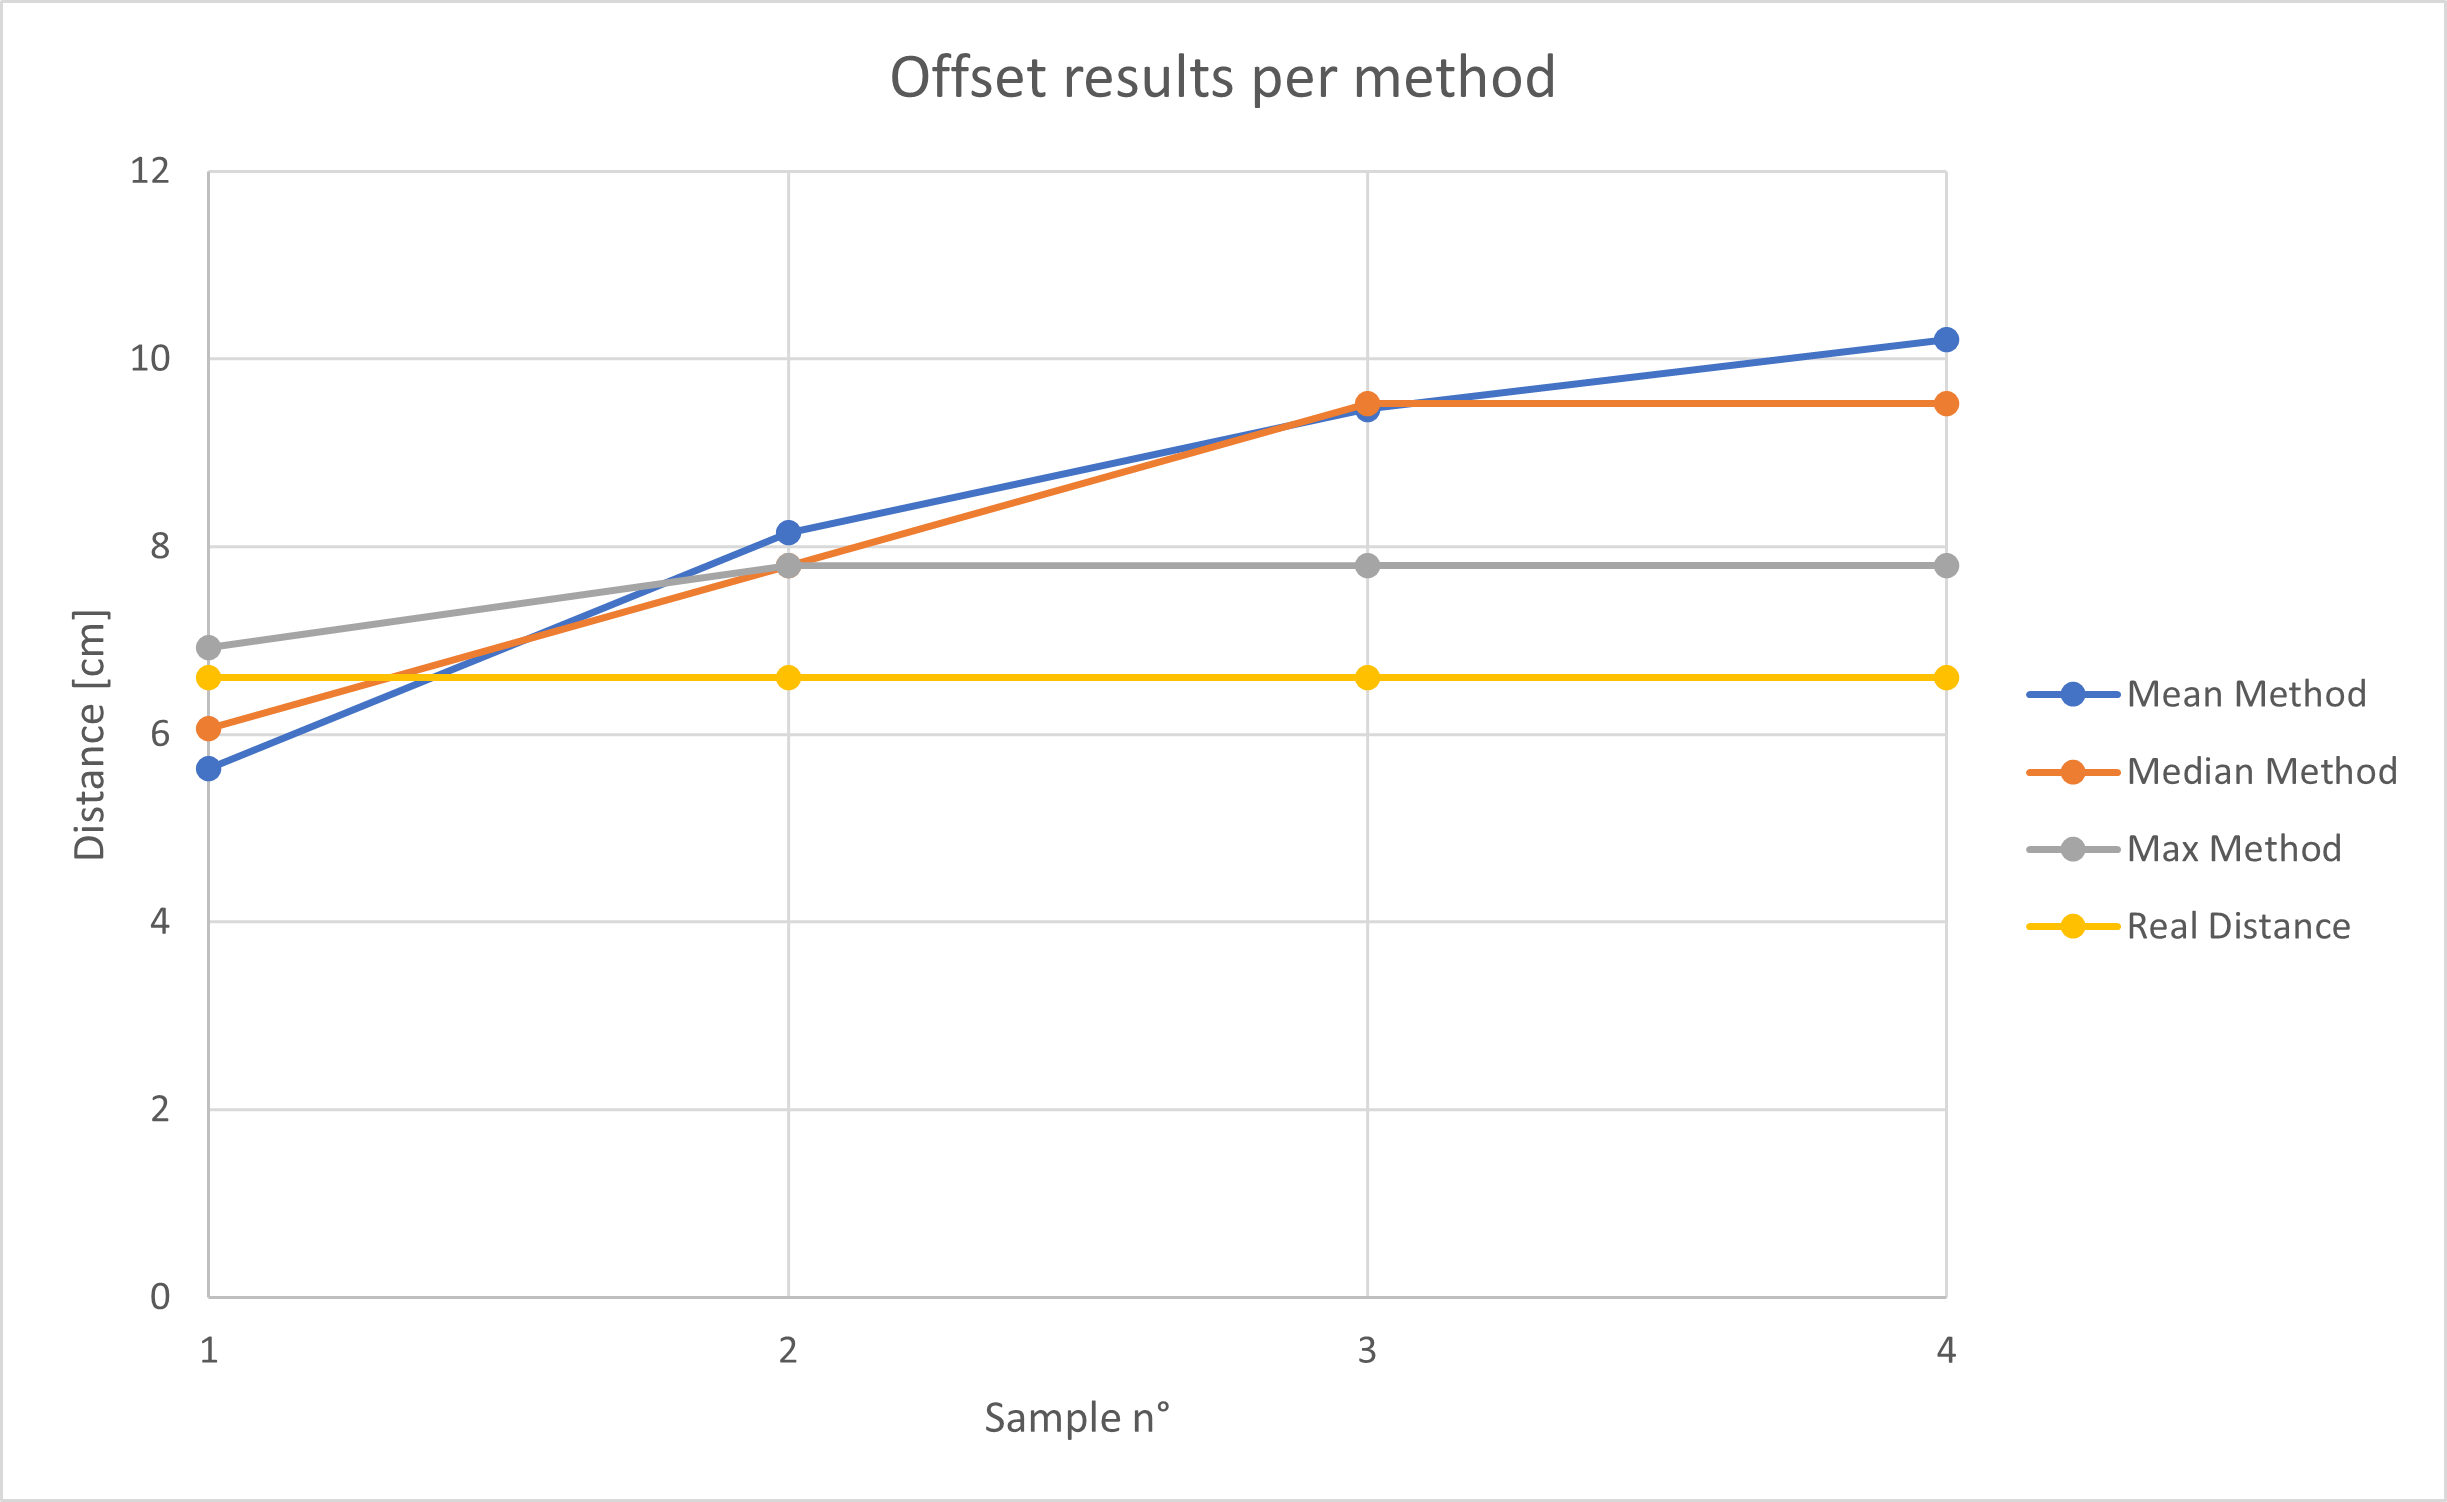
\includegraphics[width=0.8\textwidth]{Images/LiDAR/LiDAR_OffsetMes_PerMethods.png}
    \caption{Résultat des calculs d'offset par méthode}
    \label{OffsetMes_PerMethod}
\end{figure}

\subsubsection{Conclusion préliminaire} 

Le graphe \ref{OffsetMes_Moustache} montre la répartition des mesures effectuées sous la forme d'une
boîte à moustache. Cela permet de représenter facilement la répartition des mesures autour de la médiane.\\
On remarque sur les séries \emph{Noise 1} à \emph{Noise 3} que du bruit a bien été généré par les
opérateurs, ce qui n'est pas le cas pour les deux premières séquences de mesure. Hormis cela, le graphe
est très similaire aux tests dans un environnement perturbé, à la section \ref{MesNoise}. On retrouve
en effet une médiane qui s'éloigne de plus en plus de la vraie distance, alors que le maximum s'approche
le plus de la réalité.\par
On voit sur la figure \ref{OffsetMes_PerMethod} l'épaisseur calculée à l'aide de la méthode de la section
\ref{MethodeDeMesure} pour les 3 solutions proposées, à savoir la moyenne, la médiane et le maximum. Ce
calcul d'offset a été réalisé pour les quatre séries de mesures à disposition, avec un bruit graduel. On 
peut ici conclure que la méthode du maximum est la plus proche de la réalité. Pour cette raison, elle sera
utilisée pour les tests sur le terrain.

\subsection{Mesure de hauteur en situation réelle}

Après avoir prouvé le fonctionnement du capteur en laboratoire, il est essentiel de le tester en conditions
réelles, sous la neige. Pour ce faire, des tests ont été réalisés la nuit du 3 au 4 décembre 2021 à Ayent.
Un boitier temporaire a été confectionné afin de protéger le LiDAR et la carte de développement des 
précipitations.

\subsubsection{Méthode}

Le boitier a été installé sur un trépied à 140cm au-dessus du sol, sous un couvert, à l'abri de la majorité
des flocons. Le LiDAR pointe vers le sol avec un angle de 45° par rapport à la verticale, donnant une
distance de 197cm entre le capteur et la route. Les données récoltées sont enregistrées via un câble 
USB sur un ordinateur.\\
Le but est de mesurer des épaisseurs de neige en partant de 0cm (la route a été nettoyée au préalable)
afin de mettre à l'épreuve l'efficacité du capteur et de nos méthodes de mesure. Chaque mesure d'épaisseur 
est réalisée chaque 30 secondes, et ce pendant plus d'une heure. En parallèle, une double-mètre est posé 
dans la neige afin de relever périodiquement la hauteur de neige présente sur la route. Une mesure
qualitative du débit de neige est aussi effectuée. La figure \ref{RealTest_Setup} montre la mise en
place du test. Le double-mètre et l'ordinateur ne sont pas visibles ici.

\begin{figure}[H]
    \centering
    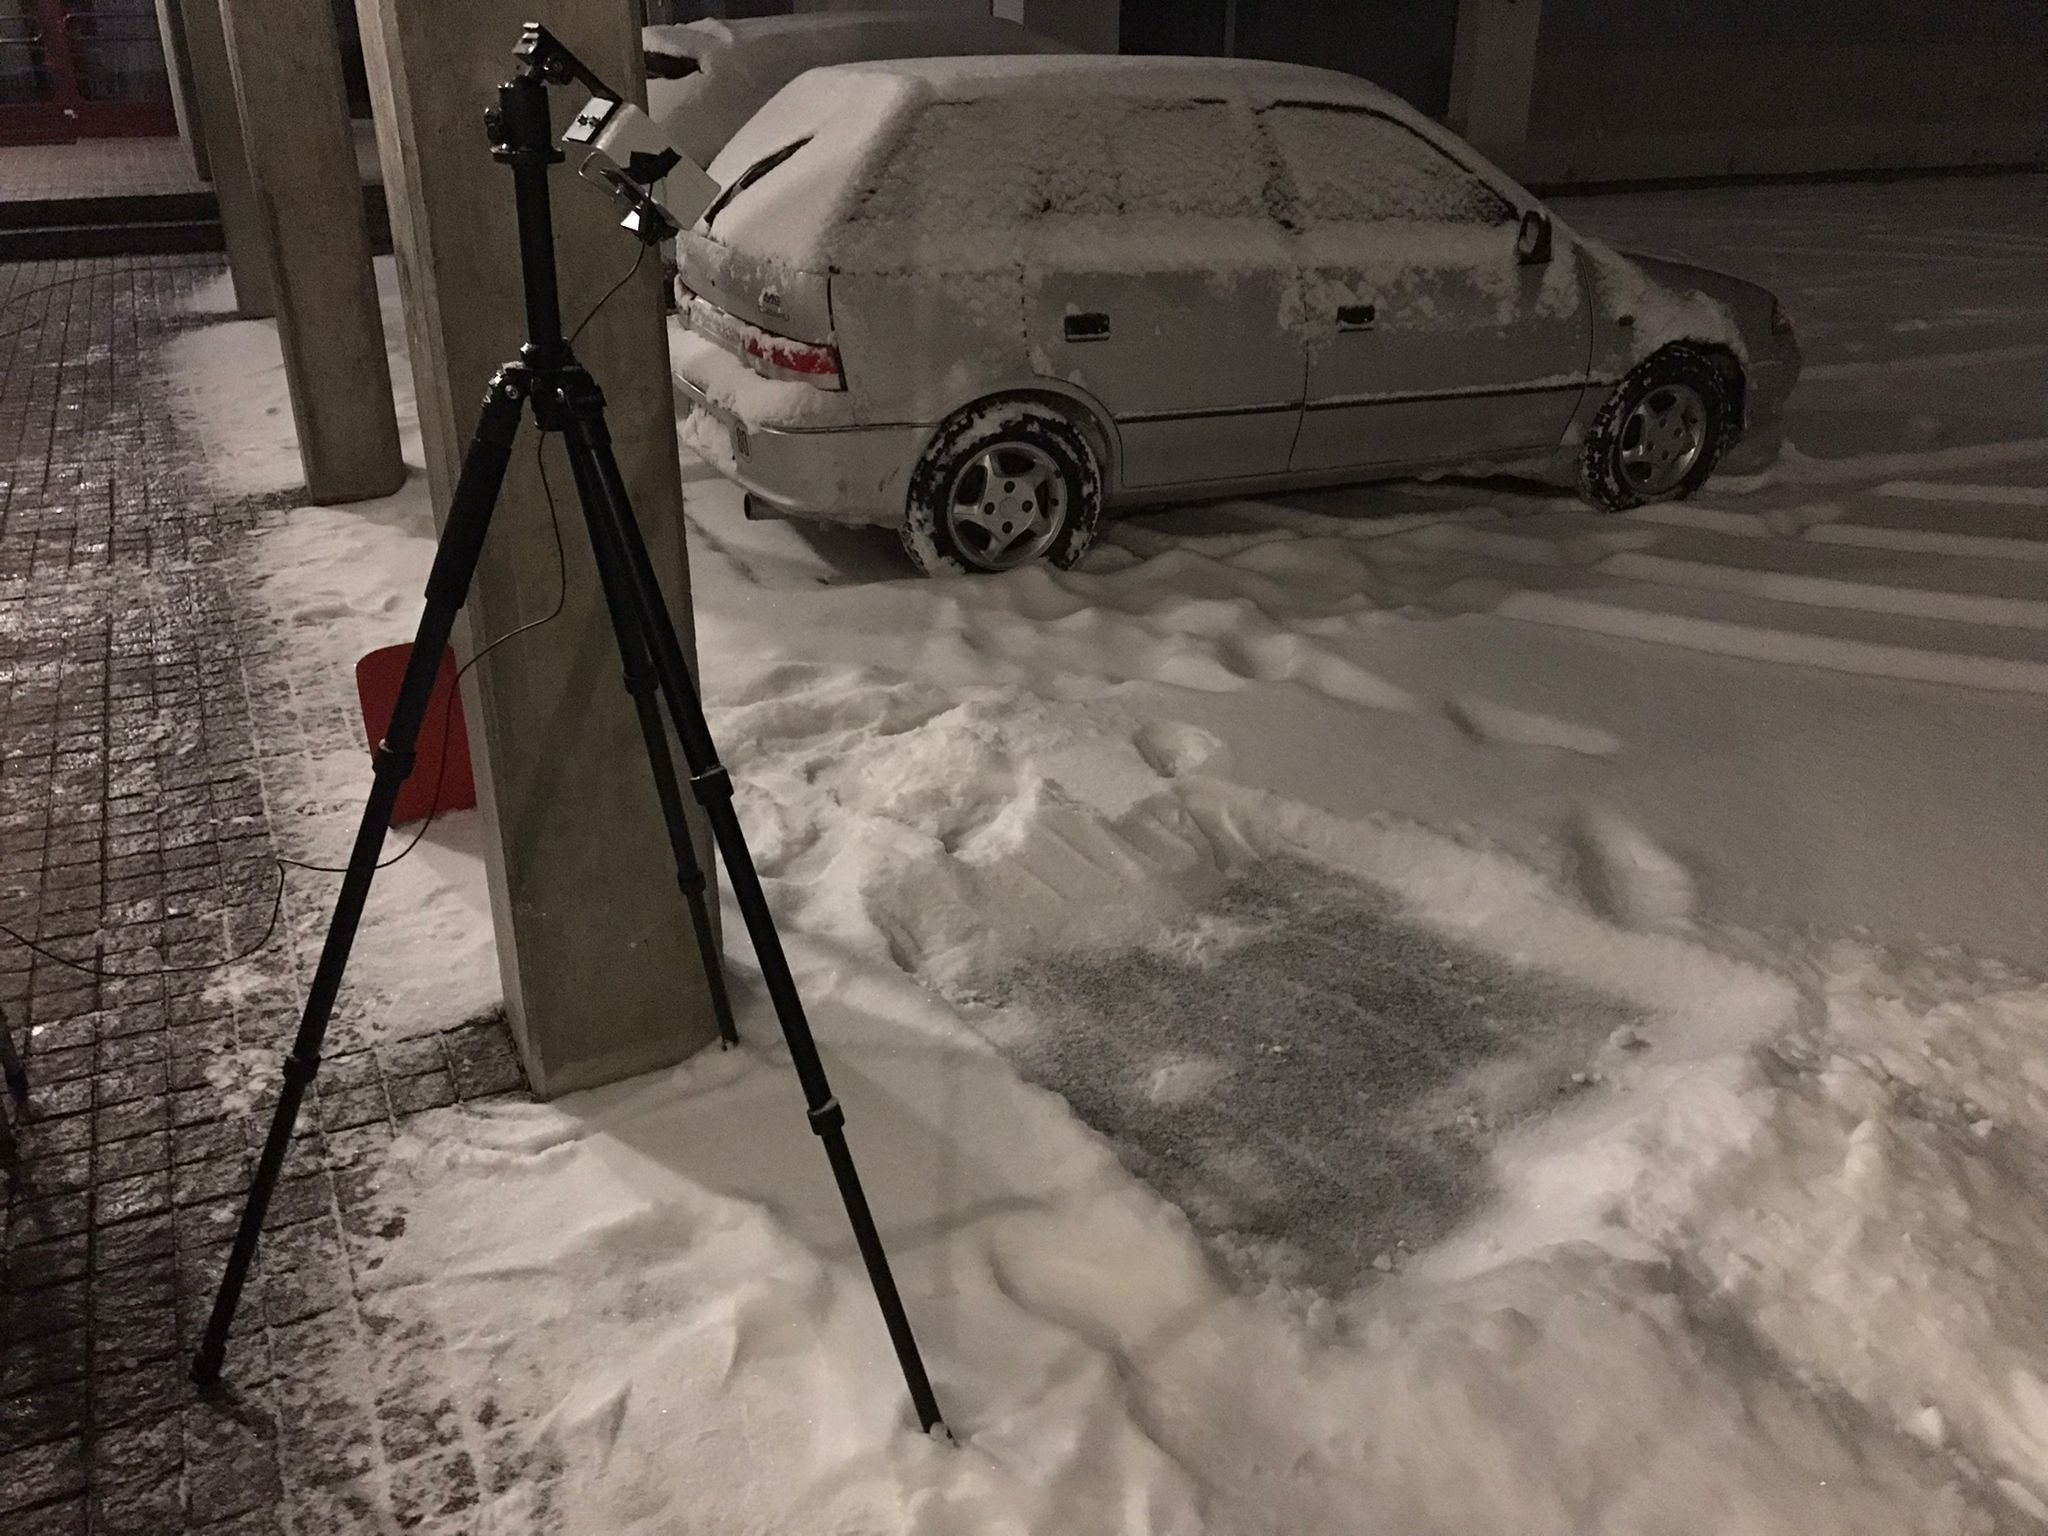
\includegraphics[width=0.75\textwidth]{Images/LiDAR/ReadTests_Setup.jpeg}
    \caption{Mise en place du test en condition réelle}
    \label{RealTest_Setup}
\end{figure}

\subsubsection{Résultats du test}

\begin{table}[H]
    \centering
    \begin{tabular}{|c|c|c|c|c|}
        \hline
        Mesure n° & Hauteur réelle [cm] & Hauteur mesurée [cm] & Type de précipitation & Heure \\
        \hline\hline
        1 & 0 & 0 & Petits flocons & 04h28 \\
        \hline
        2 & 0.5 & 0.71 & Petits flocons & 04h39 \\
        \hline
        3 & 0.8 & 1.41 & Quelques gros flocons & 04h48 \\
        \hline
        4 & 1.5 & 1.41 & Quelques gros flocons & 05h00 \\
        \hline
        5 & 2 & 2.12 & Quelques gros flocons & 05h08 \\
        \hline
        6 & 2.5 & 2.12 & Quelques gros flocons & 05h14 \\
        \hline
        7 & 2.8 & 2.86 & Quelques gros flocons & 05h21 \\
        \hline
        8 & 3 & 2.86 & Quelques gros flocons & 05h32 \\
        \hline
        
    \end{tabular}
    \caption{Mesures relevée lors du test}
    \label{SnowingState}
\end{table}

\begin{figure}[H]
    \centering
    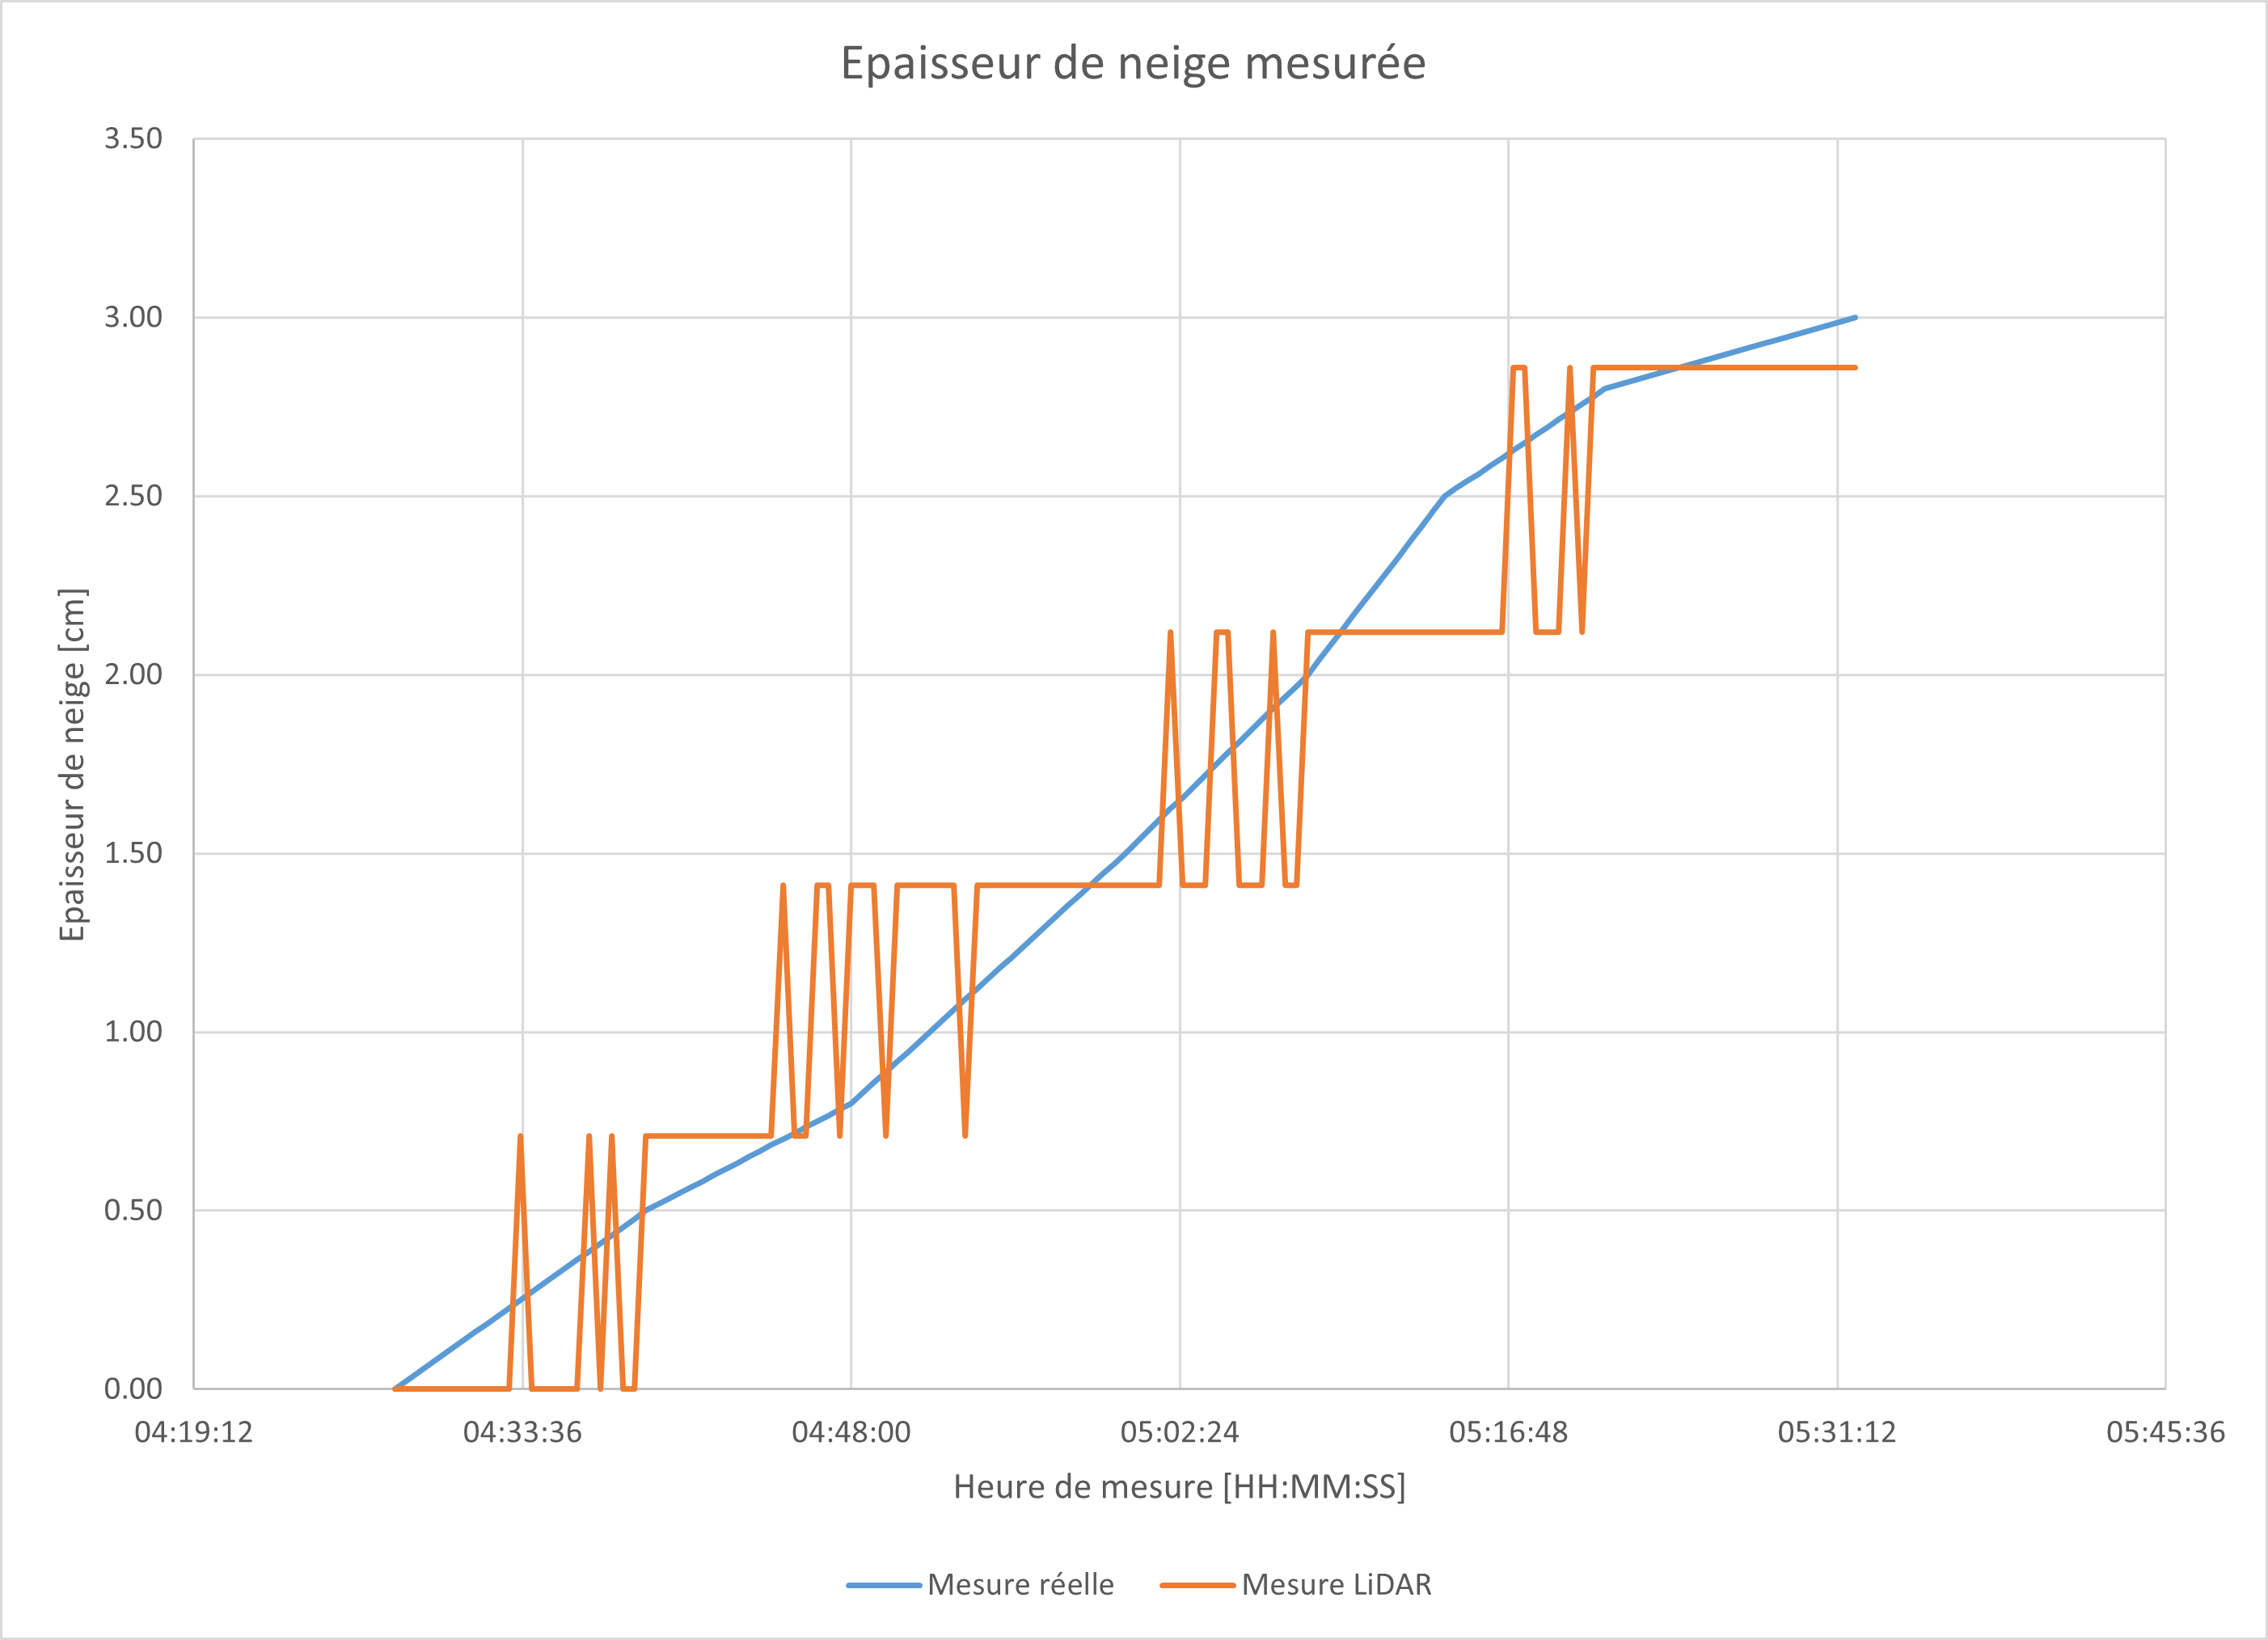
\includegraphics[width=0.75\textwidth]{Images/LiDAR/ReadTests_Results.png}
    \caption{Résultat des mesures effectuées}
    \label{RealTest_Results}
\end{figure}

La température lors des mesures oscillait entre -2°C et 0°C, sans aucun vent.\par 
Afin de réaliser la courbe \emph{Mesure réelle} de la figure \ref{RealTest_Results}, une interpolation
linéaire a été utilisée entre les différents points de mesure.

\subsubsection{Conclusion préliminaire} 

Après avoir passé plusieurs heures dans un froid glacial à mettre à l'épreuve notre projet, nous avons 
enfin pu obtenir des résultats.\\
Le tableau \ref{SnowingState} montre les différentes heures de mesures, mettant notamment en évidence
l'erreur entre la valeur réelle et mesurée. Malgré une légère oscillation lors d'un changement proche
de valeur (figure \ref{RealTest_Results}), on peut conclure que le LiDAR arrive bel et bien à mesurer 
une hauteur de neige, et ce depuis le sol.\par 
On constate par la même occasion que le pas de mesure du capteur dépend effectivement de son angle par 
rapport à la verticale.